\chapter{Results}
\label{chapterlabel5}

The aim of this section is to both test the proposed parallel imaging pipeline and the SENSE reconstruction algorithm for different scenarios. First, the proposed pMRI technique is performed using an acceleration factor $R = 1$ (no phase-encoding lines are skipped) for all defined sensitivity maps and for all previously described coil configurations. Second, the quality of reconstruction is tested for increasing acceleration factors. Finally, the outcome of the reconstruction when increasing levels of noise are added to the sensitivity profiles is presented. 
%Finally, motion during acquisition time is considered and the proposed pipeline is again investigated. 

%%%%%%%%%%%%%%
\section{Enhancing POSSUM with multi-coil acquisition}
This section is concerned with the proposed multi-coil acquisition pipeline. First, the design of the experiment is presented, followed by results and further discussion.

\subsection{Design}
The first step towards enhancing POSSUM with parallel imaging capabilities is to enable it to receive as input the sensitivity maps of the coils. For this reason, the current section is concerned with generating the coil sensitivity profiles for all subsequent simulations. Moreover, SENSE reconstructions will be performed without skipping phase-encoding lines (full FOV images).

As stated before, the object used as input in POSSUM, representing a brain, consists of 192 x 192 x 192 cuboid elements, with physical dimensions of 1mm x 1mm x 1mm, containing information about the properties (spin density $\rho$, $T_1$ and $T_2^*$ relaxation times) of each tissue type (WM, GM and CSF). For this reason, the sensitivity maps of each receiver channel were generated to be of the same size as the input object and to contain, for each voxel within, a value between 0 and 1 representing the sensitivity of the signal originating from that particular spatial location (a value of 1 represents maximum sensitivity, whereas for 0 no signal is perceived).

In compliance with realistic sensitivity profiles, the design of choice was to enforce the spatial variations of the sensitivity values to take a 2 dimensional Gaussian form of isotropic cross-section. Various standard deviations of the normal distribution were used to generate the sensitivity profiles, while different channel combinations were generated by shifting the center of the Gaussian to a different spatial location within a slice. 

Under these circumstances, the parallel imaging pipeline was tested with 2, 4, 6, 8, 12 and 16 phased-array coil combinations for various standard deviations of the normal distributions ranging from 6 to 96. The results are shown in the following section.

\subsection{Results}
Figure~\ref{fig:1coildifsigmas2} shows the coil sensitivity profiles as generated for this project. For qualitative reasons, the sensitivity profiles have been overlaid on top of the object of interest (the brain used as input for our simulations). As stated before, we have chosen to spatially vary their sensitivities by modelling normal distributions of various standard deviations. The $\sigma$ values go from $6$ to $96$. As can be seen, higher standard deviations will translate into more field-of-view coverage, while a lower standard deviation will only affect part of the domain. 

In order to test the reconstruction accuracy, we have chosen to create various arrangements of these sensitivity profiles. In all of our subsequent simulations, the number of channels chosen were: 2, 4, 6, 8, 12 and 16. Figure~\ref{fig:2coilsdifsigmas2} shows the 2-channel arrangement while the others are presented in Appendix~\ref{appendixlabel1}.

\begin{figure}[H]
    \centering
    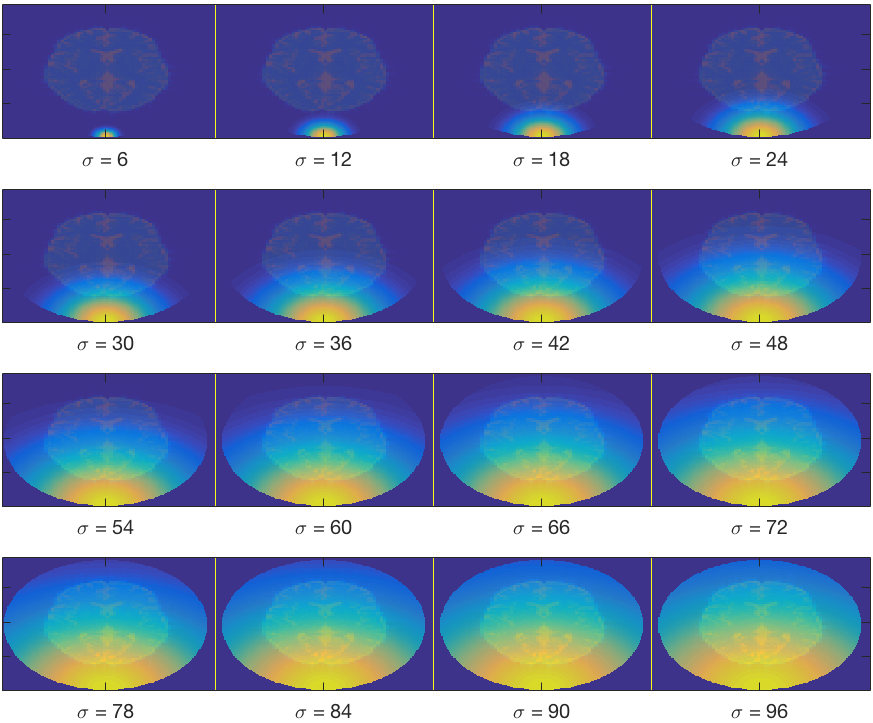
\includegraphics[width=.85\textwidth,keepaspectratio]{1coildifsigmas}
    \caption{Coil sensitivity profiles used in simulations}
    \label{fig:1coildifsigmas2}
\end{figure}

\begin{figure}[H]
    \centering
    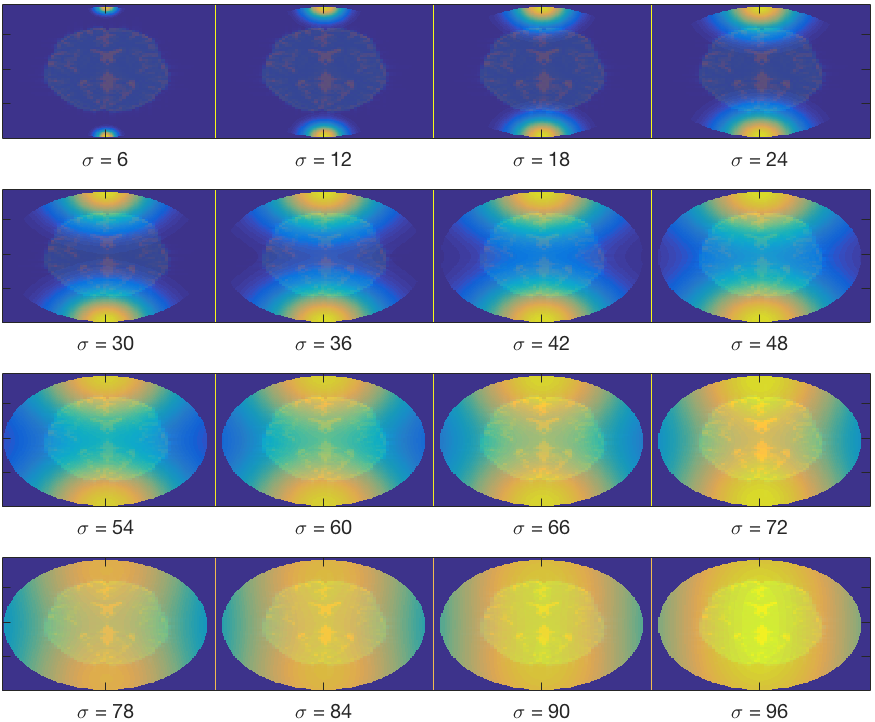
\includegraphics[width=.85\textwidth,keepaspectratio]{2coilsdifsigmas}
    \caption{Coil sensitivity maps of the 2-channel phased-array coil}
    \label{fig:2coilsdifsigmas2}
\end{figure}

All of the presented maps have been used as inputs to POSSUM in order to generate \textit{sensitivity-weighted} reconstructions. Due to the increasing computational time as the number of channels gets higher, the design of choice was to run POSSUM for each sensitivity map independently. This allows for faster simulations as on a cluster system each coil will be treated by a different job, in parallel. Moreover, the complexity of the array (coil location and number of channels) will not influence the running time significantly.

\begin{figure}[H]
    \centering
    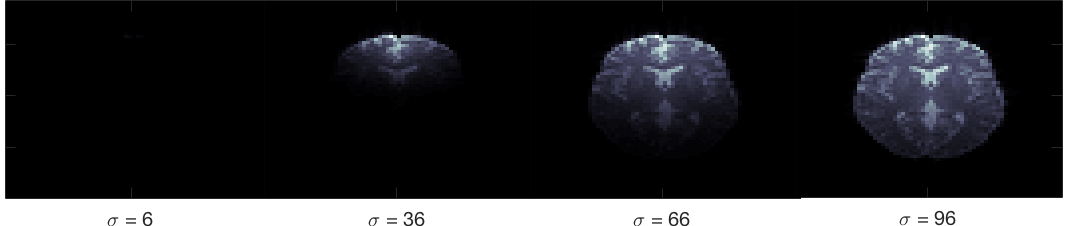
\includegraphics[width=1\textwidth,keepaspectratio]{brainsdifsigmas}
    \caption{Results of POSSUM enhanced simulations for increasing standard deviations of the sensitivity profiles of one channel}
    \label{fig:brainsdifsigmas}
\end{figure}

Figure~\ref{fig:brainsdifsigmas} shows the output of 4 simulations which were run for 4 of the previously described sensitivity maps. The lowest and highest standard deviations used are shown in this figure to better visualise the two extremes. Moreover, the figure only shows one output image per simulation corresponding to a coil positioned in the upper part of the object. Reconstructions of the final images given all coil combinations and different sensitivity maps are presented in Figure~\ref{fig:1brainsR1rec}. To better visualise the quality of reconstruction, Figure~\ref{fig:1brainsR1ssd} shows the sum of squared differences between each reconstruction and the original image. The latter was simulated with the equivalent of a homogeneous sensitivity map and with full FOV acquisition.

\subsection{Discussion}
In this first experiment we showed that multi-coil acquisition is now possible with POSSUM. The first step towards this goal was to create a collection of different sensitivity maps showing different amounts of object coverage in terms of coil sensitivity. SENSE reconstruction was also performed with $R = 1$ as was described in Section~\ref{ch4sectionsense}. 

Figure \ref{fig:1brainsR1rec} shows the SENSE reconstructions performed for increasing standard deviations of the sensitivity profiles and for all coil combinations. The trend shows an increased performance as coil geometry gets better. For example, for a 2-channel array, the algorithm is unable to reconstruct the image for the same sensitivity profile used in the 4/6/8/12/16-channel arrays. Moreover, a convergence seems to be reached in the last column, where all coil combinations perform well. This is backed up by Figure \ref{fig:1brainsR1ssd} which shows a similar trend. 

\begin{figure}[H]
    \centering
    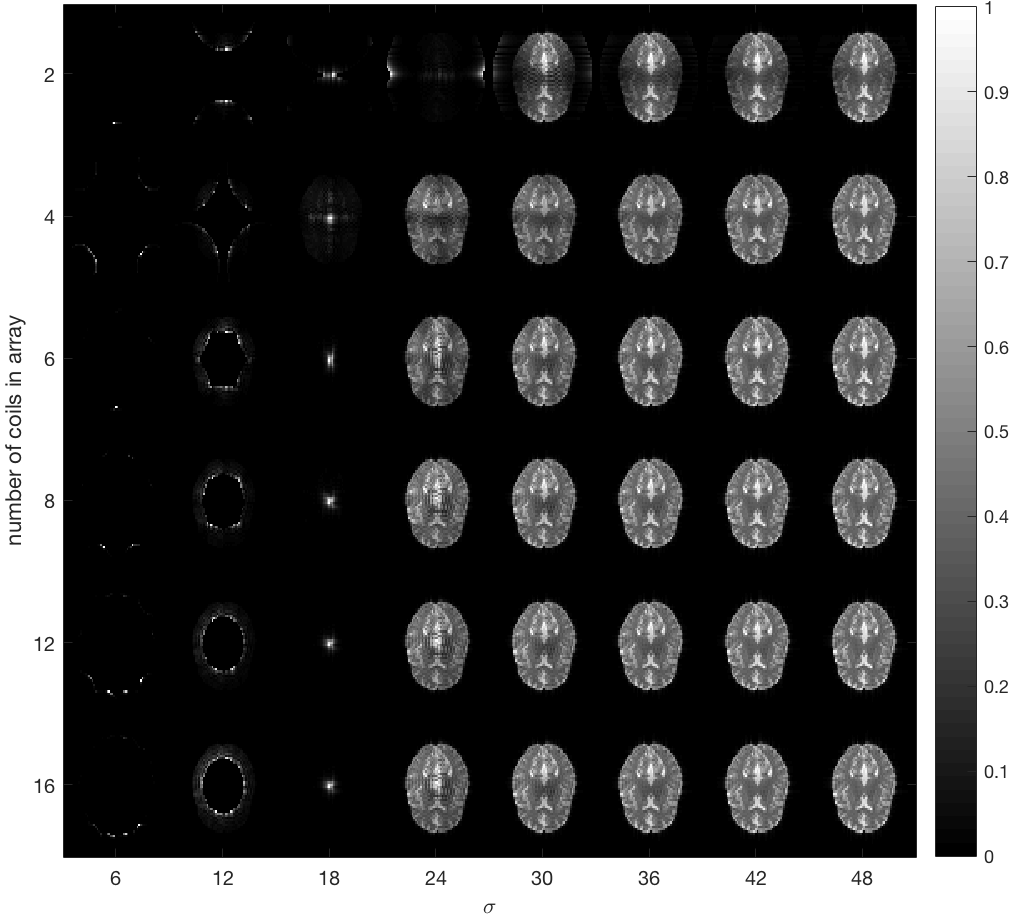
\includegraphics[width=1\textwidth,keepaspectratio]{1brainsR1rec}
    \caption{Reconstruction of multi-coil acquisitions for different numbers of channels and for different standard deviations of the associated sensitivity maps}
    \label{fig:1brainsR1rec}
\end{figure}

In conclusion, this first experiment tells us that multi-coil acquisition requires a good combination of at least two parameters: the standard deviation of the associated sensitivity map and the geometry of the coil array. As can be seen in Figures \ref{fig:1brainsR1rec} and \ref{fig:1brainsR1ssd}, choosing small standard deviations of the sensitivity profiles will translate into poor or even impossible reconstructions. However, in parallel imaging techniques, too much coverage can also be detrimental as in that case distinguishing between two or more spatial locations would become impossible. This happens because a very smooth sensitivity profile used in conjunction with a high number of channels can mean that many spatial locations within the object of interest will be "weighted" by the same sensitivity value. This will lead to incorrect reconstructions. In the following section, different acceleration factors are considered and SENSE reconstruction is again performed.

\begin{figure}[H]
    \centering
    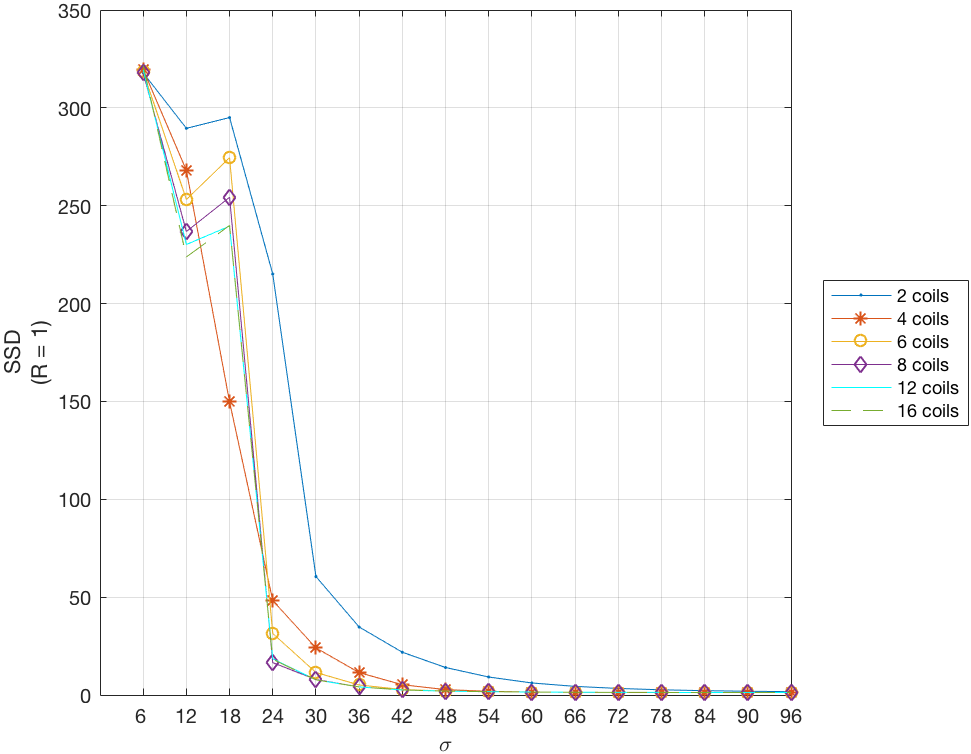
\includegraphics[width=1\textwidth,keepaspectratio]{1brainR1ssd}
    \caption{SSD between original image and the reconstructions coming from each multi-coil acquisitions for different numbers of channels and for different standard deviations of the associated sensitivity maps. The acceleration factor used is $R = 1$. The trend of the plot clearly shows an improvement in reconstruction as the standard deviation of the sensitivity profile and also as the number of channels in the array gets higher.}
    \label{fig:1brainsR1ssd}
\end{figure}

%%%%%%%%%%%%%%%
\section{SENSE reconstructions with different acceleration factors} \label{exp2}
This section is concerned with reconstructions performed with different acceleration factors, more specifically: $R = \left\{1, 2, 3, 4\right\}$. The aim of this experiment is to investigate how the quality of reconstruction is affected by increasing acceleration factors. The experiment design will be discussed first, followed by results and discussion.

\subsection{Design}
The next step towards implementing a parallel imaging pipeline in POSSUM is to enable simulations with undersampled acquisitions in the phase-encoding direction. The method of choice and its implementation in POSSUM was detailed in Section~\ref{ch4sectionaliased}. 

For this experiment 4 acceleration factors, more specifically $R = \left\{1, 2, 3, 4\right\}$, were considered. The sequence under test was an EPI sequence with a $N_x$ x $N_y$ of 64 x 64 sampling steps. In our case, this means that the number of phase-encoding lines acquired was decreased from a full 64 line acquisition, to 32 lines for $R = 2$, to 21 lines for $R = 3$, and, finally, 16 lines when $R = 4$. Higher acceleration factors were not taken into consideration as the amount of information left would have been too low for good reconstructions and are generally not used in clinical practices.

For each of these, simulations were run for all channel array combinations and for all sensitivity profiles presented before, with reconstructions shown in the next subsection. Moreover, as the quality of reconstruction depends on the coil "g-factor", this was also calculated for all possible combinations. As stated before, the "g-factor" is a measure of noise amplification at a given location in the final image and is, therefore, a location-specific indication of how well the signal can be retrieved given a specific coil combination and a certain acceleration factor.

\begin{figure}[H]
    \centering
    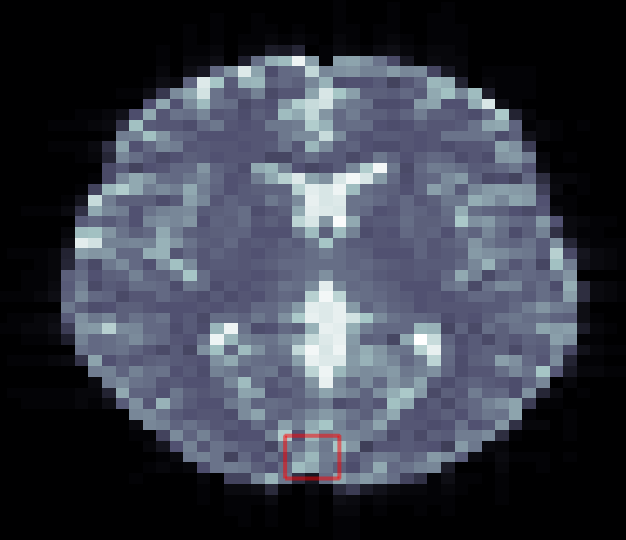
\includegraphics[width=.3\textwidth,keepaspectratio]{roigfact}
    \caption{The chosen ROI for the g-factor calculations}
    \label{fig:roigfact}
\end{figure}

Finally, a region of interest was considered (see Figure~\ref{fig:roigfact}) and the "g-factor", together with the relative decrease in signal-to-noise ratio, was calculated for all coil arrays and all sensitivity profiles.

\subsection{Results}
As stated before, this experiment is focused on the quality of reconstruction for different acceleration factors. Figures \ref{fig:R1brains}, \ref{fig:R2brains}, \ref{fig:R3brains} and \ref{fig:R4brains} show SENSE reconstructions for different acceleration factors, while Figures \ref{fig:R1gfact}, \ref{fig:R2gfact}, \ref{fig:R3gfact} and \ref{fig:R4gfact} show their associated "g-factor" maps.

For visualisation purposes, all "g-factor" maps have been normalised. Still, it is visible from the figures that increasing numbers of coils and also increasing coverage values of the sensitivity profiles will contribute with more uncertainty in the final images as can be seen from the "g-factor" maps and reconstruction figures. 

In addition to qualitatively assessing the reconstructions, a sum-of-squared differences was performed between each SENSE reconstruction and the non-aliased original image for all combinations of values. The results can be seen in Figure~\ref{fig:2SSD} where each plot is a different acceleration factor R.

A quantification of the dependency between our 3 varying parameters (number of coils, acceleration factors and standard deviations) and the quality of reconstruction is shown in Figure~\ref{fig:2gfactor}. It is visible from the plots that an increase in the number of channels used aids the reconstruction. In between plots, it is also visible that higher acceleration factors will decrease the subsequent quality of reconstruction, with a higher plateau reached as $R$ increases. This is due to the fact that when high acceleration factors are used in combination with an increased number of coils, the reconstruction becomes ill-conditioned.

As stated before, the g-factor values also contribute to the overall SNR of the reconstruction. Knowing that $SNR_{SENSE} = \frac{SNR_{Original}}{g \sqrt{R}}$, a region of interest was chosen to calculate the drop in relative SNR due to increasing acceleration factors and, hence, noise contribution coming from different coils. Figure \ref{fig:2SNRsense} shows these results. Again, all three parameters influence the quality of reconstruction. 

%% R1
\begin{figure}[H]
    \centering
    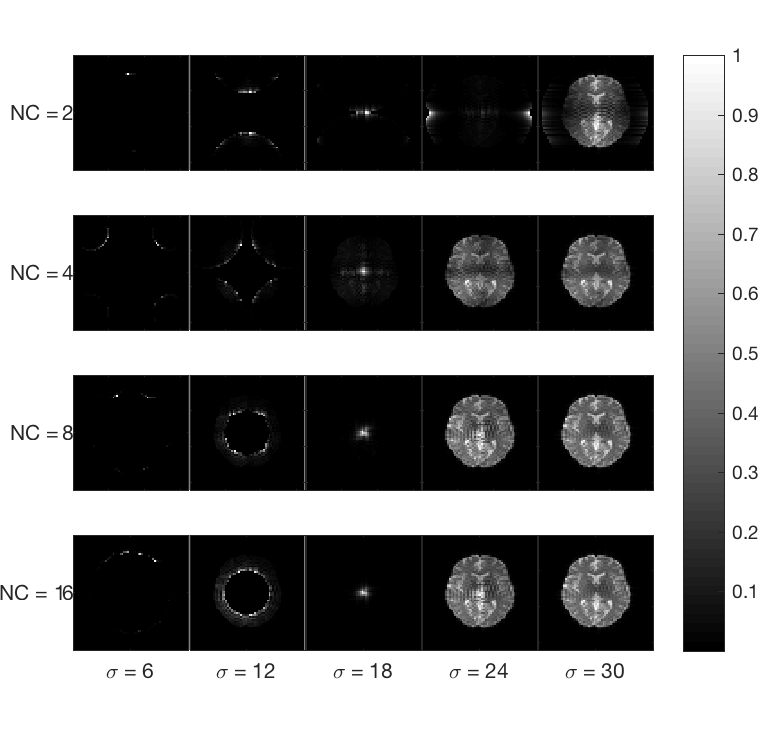
\includegraphics[width=1\textwidth,keepaspectratio]{R1brainsb}
    \caption{SENSE reconstructions for acceleration factor $R = 1$, for increasing numbers of coils on the y-axis and with varying standard deviations of their associated sensitivity profiles on the x-axis}
    \label{fig:R1brains}
\end{figure}

\begin{figure}[H]
    \centering
    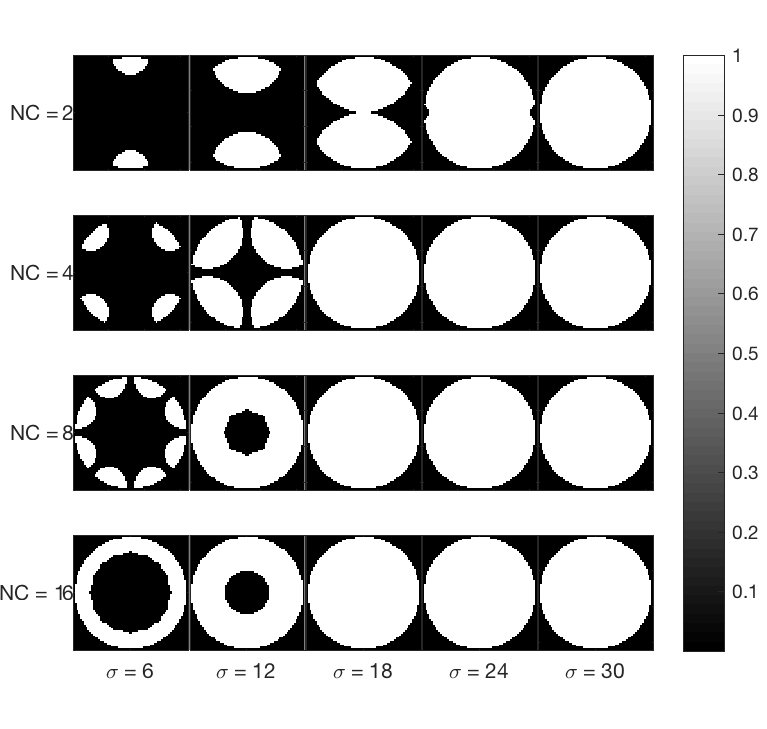
\includegraphics[width=1\textwidth,keepaspectratio]{R1gfactb}
    \caption{g-factor maps for acceleration factor $R = 1$, for increasing numbers of coils on the y-axis and with varying standard deviations of their associated sensitivity profiles on the x-axis}
    \label{fig:R1gfact}
\end{figure}

%% R2
\begin{figure}[H]
    \centering
    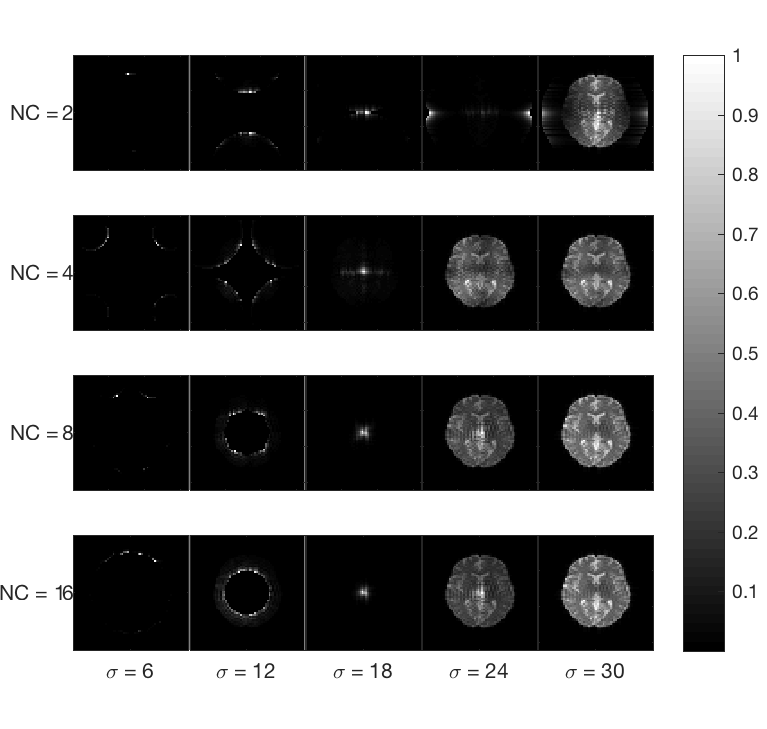
\includegraphics[width=1\textwidth,keepaspectratio]{R2brainsb}
    \caption{SENSE reconstructions for acceleration factor $R = 2$, for increasing numbers of coils on the y-axis and with varying standard deviations of their associated sensitivity profiles on the x-axis}
    \label{fig:R2brains}
\end{figure}

\begin{figure}[H]
    \centering
    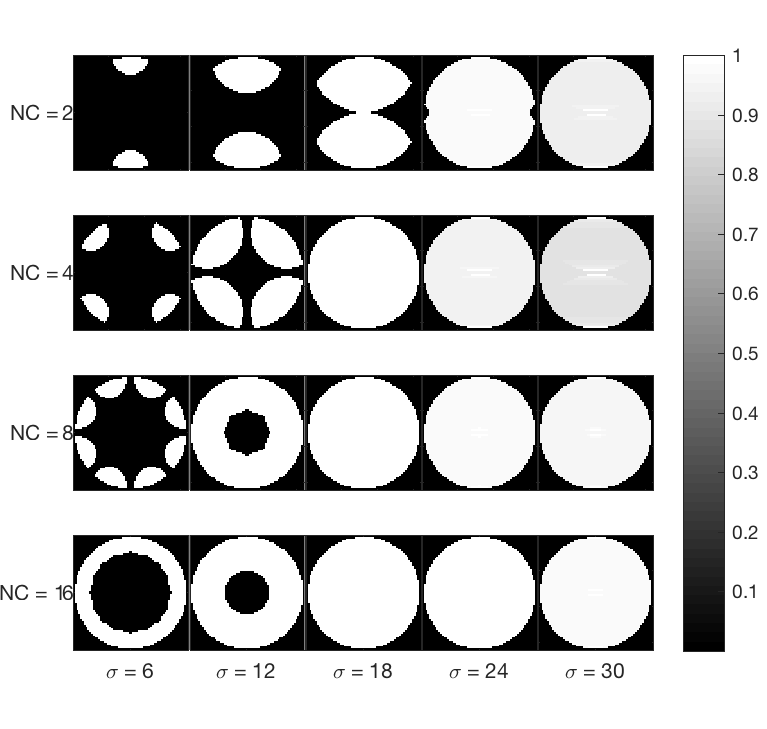
\includegraphics[width=1\textwidth,keepaspectratio]{R2gfactb}
    \caption{g-factor maps for acceleration factor $R = 2$, for increasing numbers of coils on the y-axis and with varying standard deviations of their associated sensitivity profiles on the x-axis}
    \label{fig:R2gfact}
\end{figure}

\subsection{Discussion}
In this experiment we have seen how varying different parameters such as the acceleration factor $R$, the number of coils used in the array and the standard deviations of the associated sensitivity maps can affect the quality of the SENSE reconstruction. 

Now, going back to Figures \ref{fig:R1brains}, \ref{fig:R2brains}, \ref{fig:R3brains} and \ref{fig:R4brains}, which show SENSE reconstructions for increasing acceleration factors, it is interesting to visually inspect the differences between the four results. One striking difference between them is that of the appearance of \textit{residual aliasing} as R is increased. This is, in fact, the main artifact associated with parallel imaging techniques. These artifacts can generally be caused by the bright edges of the images and appear wherever the unfolding process becomes ill-conditioned. 

Moreover, the regions where these artifacts appear are also paired with a decrease in SNR. Indeed, that can be seen in all of our results: Figures \ref{fig:R1gfact}, \ref{fig:R2gfact}, \ref{fig:R3gfact} and \ref{fig:R4gfact} show the locations where the noise caused by the coil geometry is higher.

In addition, our qualitative assessments are paired with quantitative results which are shown in Figure~\ref{fig:2SSD} where each plot is the sum of squared differences between each SENSE reconstruction and the non-aliased original image for a different acceleration factor R. Besides the evident increase in SSD as the acceleration factor becomes higher (due to noise enhancement), the trend of the plot is also interesting to discuss for $R > 2$. For all coil combinations, the SSD increases when the standard deviation of the sensitivity map becomes higher showing that a higher field-of-view coverage, paired with too high acceleration factors is detrimental to reconstructions. 

Finally, Figures~\ref{fig:2gfactor} and \ref{fig:2SNRsense} show the "g-factor" value and the decrease in relative signal-to-noise ratio for all combinations of parameters for a region of interest chosen in the lower part of the brain. The same trend as before can be seen here as well: higher acceleration factors paired with higher standard deviations of the sensitivity maps will cause noise enhancement and thus a drop in SNR. As another very important aspect of parallel MRI is the coil geometry, it is also visible from the plots that the 2-coil and 4-coil arrays apparently perform better than in terms of quality of reconstruction. This is true for $R = 2$, but for higher acceleration factors both perform badly. It is only in terms of coil geometry noise amplification that they score better.

%perform better in terms of quality of reconstruction. This is due to the fact that for our simulations, an increase in the number of channels causes too much overlap between the sensitivity maps and too many pixels must be unfolded. Of course, for acceleration factors higher than the number of coils in the array, the reconstruction is impossible and the results are not meaningful.

In conclusion, it is evident from our findings that a good balance needs to be met for SENSE-type reconstructions to work. This means that in a clinical scenario a good trade-off needs to be found. If acceleration is extremely important, than the final images will suffer from low SNR values. On the other hand, if high acceleration factors are not needed, than a good geometry of the coil array is important in order to achieve high quality reconstructions.

%The following experiment will consider different levels of noise added to the sensitivity maps which are used to perform SENSE reconstructions.

%% R3
\begin{figure}[H]
    \centering
    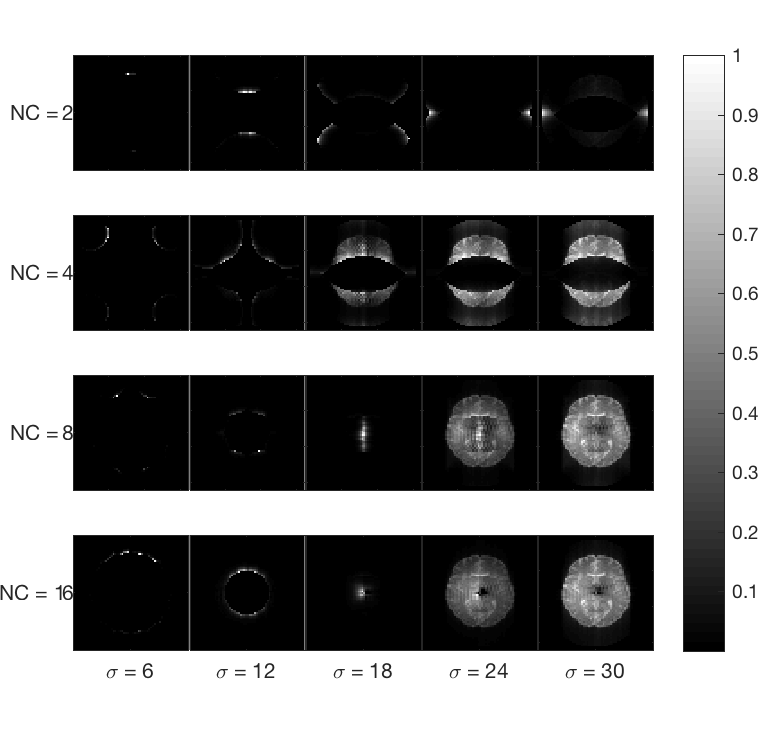
\includegraphics[width=1\textwidth,keepaspectratio]{R3brainsb}
    \caption{SENSE reconstructions for acceleration factor $R = 3$, for increasing numbers of coils on the y-axis and with varying standard deviations of their associated sensitivity profiles on the x-axis}
    \label{fig:R3brains}
\end{figure}

\begin{figure}[H]
    \centering
    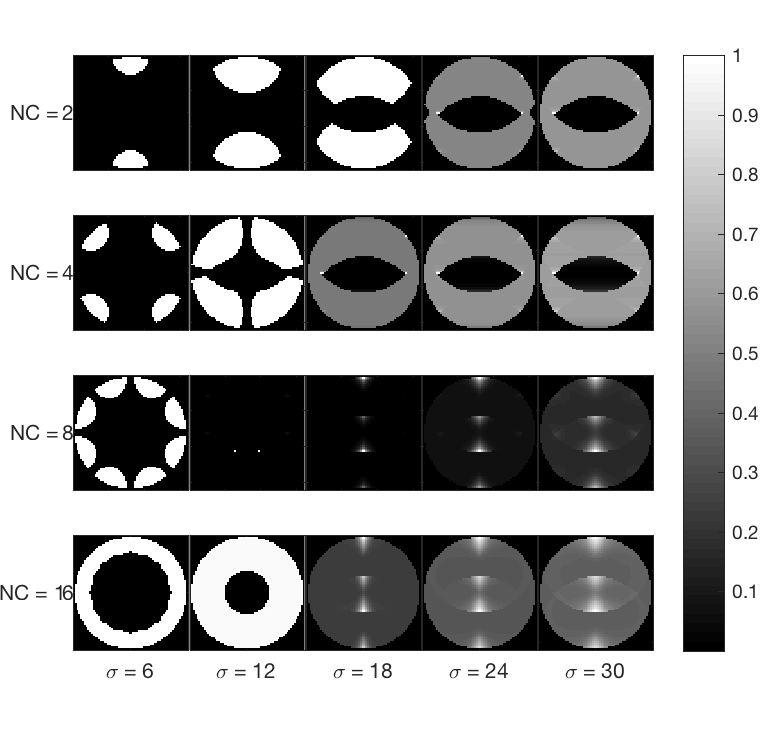
\includegraphics[width=1\textwidth,keepaspectratio]{R3gfactb}
    \caption{g-factor maps for acceleration factor $R = 3$, for increasing numbers of coils on the y-axis and with varying standard deviations of their associated sensitivity profiles on the x-axis}
    \label{fig:R3gfact}
\end{figure}

%% R4
\begin{figure}[H]
    \centering
    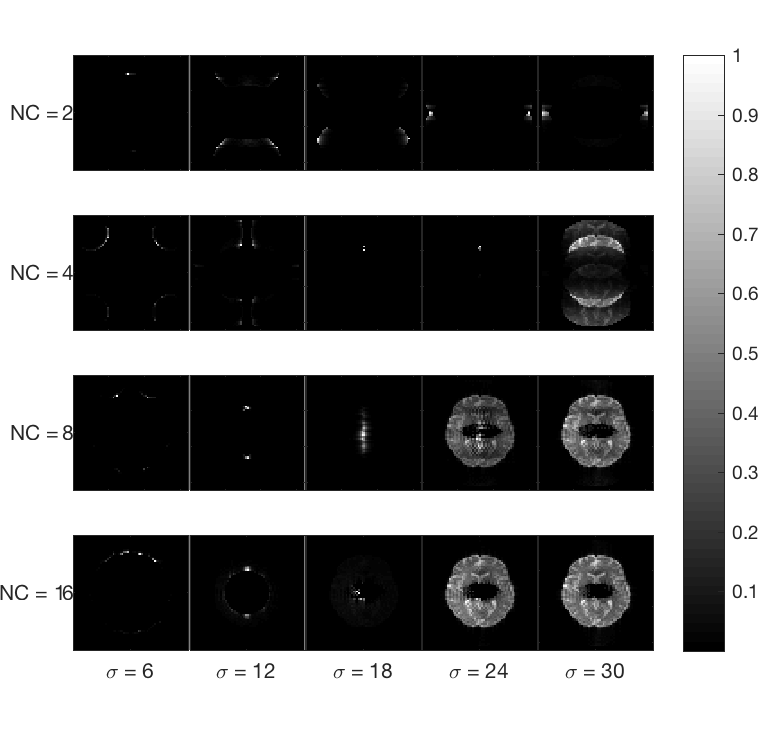
\includegraphics[width=1\textwidth,keepaspectratio]{R4brainsb}
    \caption{SENSE reconstructions for acceleration factor $R = 4$, for increasing numbers of coils on the y-axis and with varying standard deviations of their associated sensitivity profiles on the x-axis}
    \label{fig:R4brains}
\end{figure}

\begin{figure}[H]
    \centering
    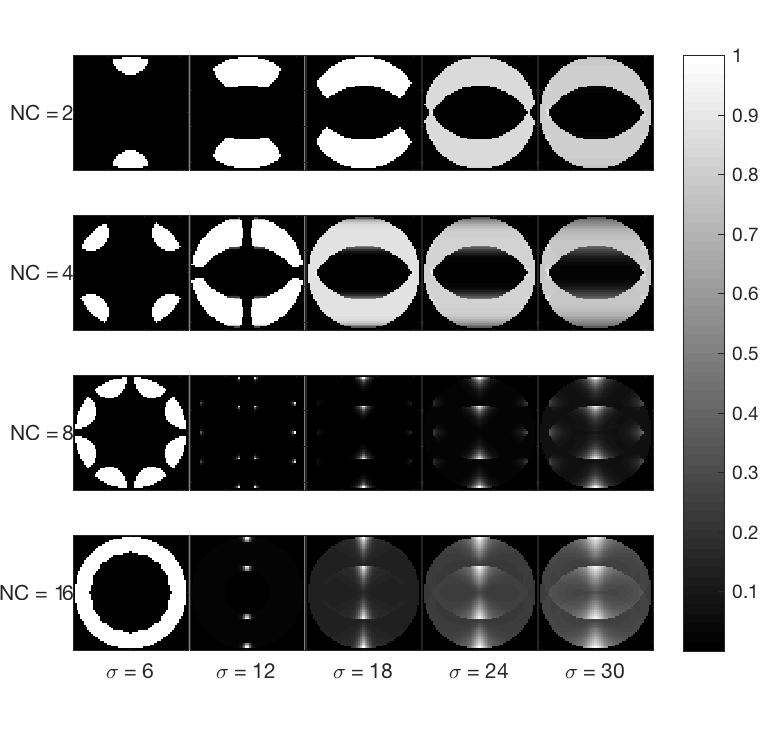
\includegraphics[width=1\textwidth,keepaspectratio]{R4gfactb}
    \caption{g-factor maps for acceleration factor $R = 4$, for increasing numbers of coils on the y-axis and with varying standard deviations of their associated sensitivity profiles on the x-axis}
    \label{fig:R4gfact}
\end{figure}

%%%%%% SSD PLOT
\begin{figure}[H]
    \centering
    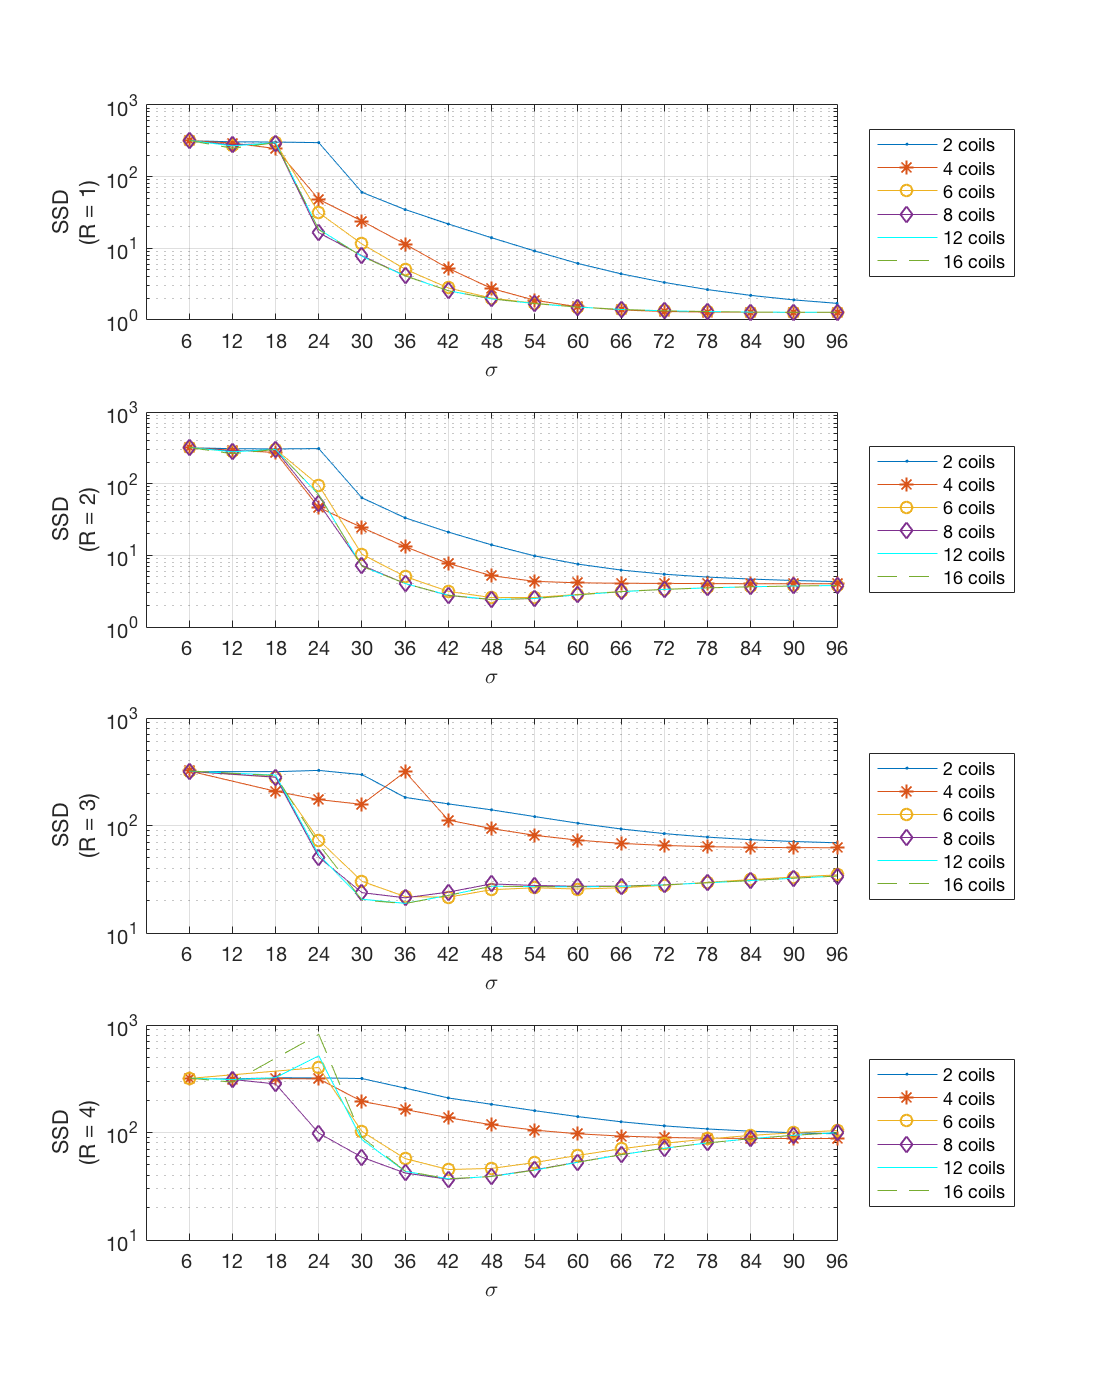
\includegraphics[width=1\textwidth,keepaspectratio]{2SSD}
    \caption{SSD for all acceleration factors, for all coil combinations and for all deviations of their associated sensitivity profiles}
    \label{fig:2SSD}
\end{figure}

\begin{figure}[H]
    \centering
    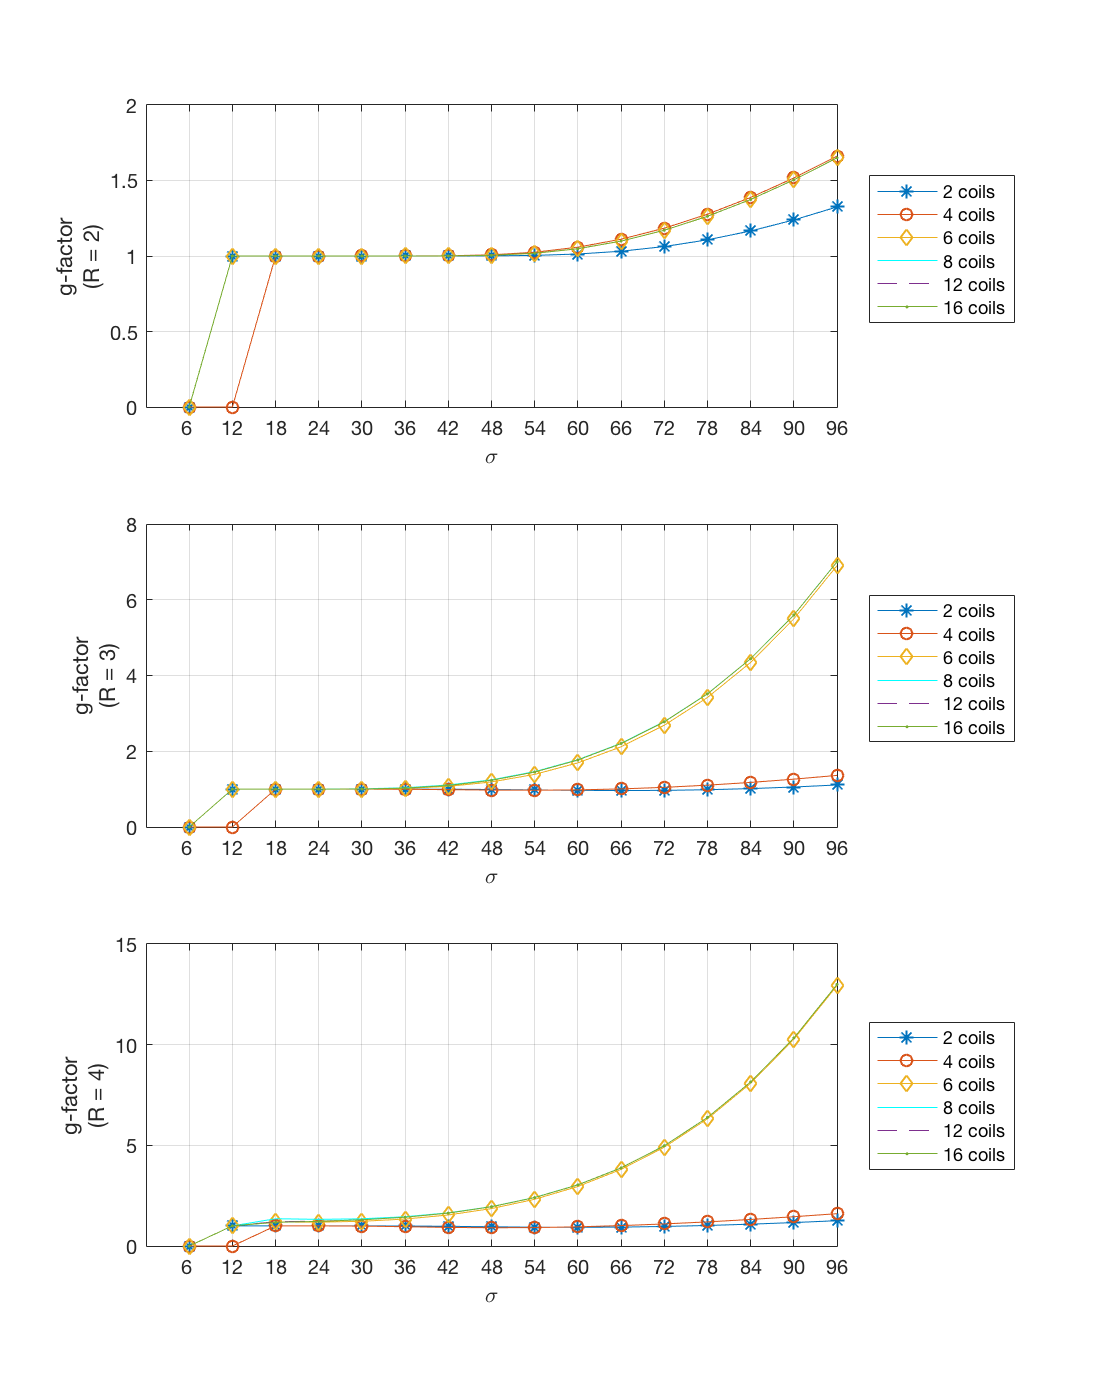
\includegraphics[width=1\textwidth,keepaspectratio]{2gfactor}
    \caption{ROI "g-factor" values for increasing acceleration factors, coil numbers and standard deviations of the associated sensitivity maps}
    \label{fig:2gfactor}
\end{figure} 

\begin{figure}[H]
    \centering
    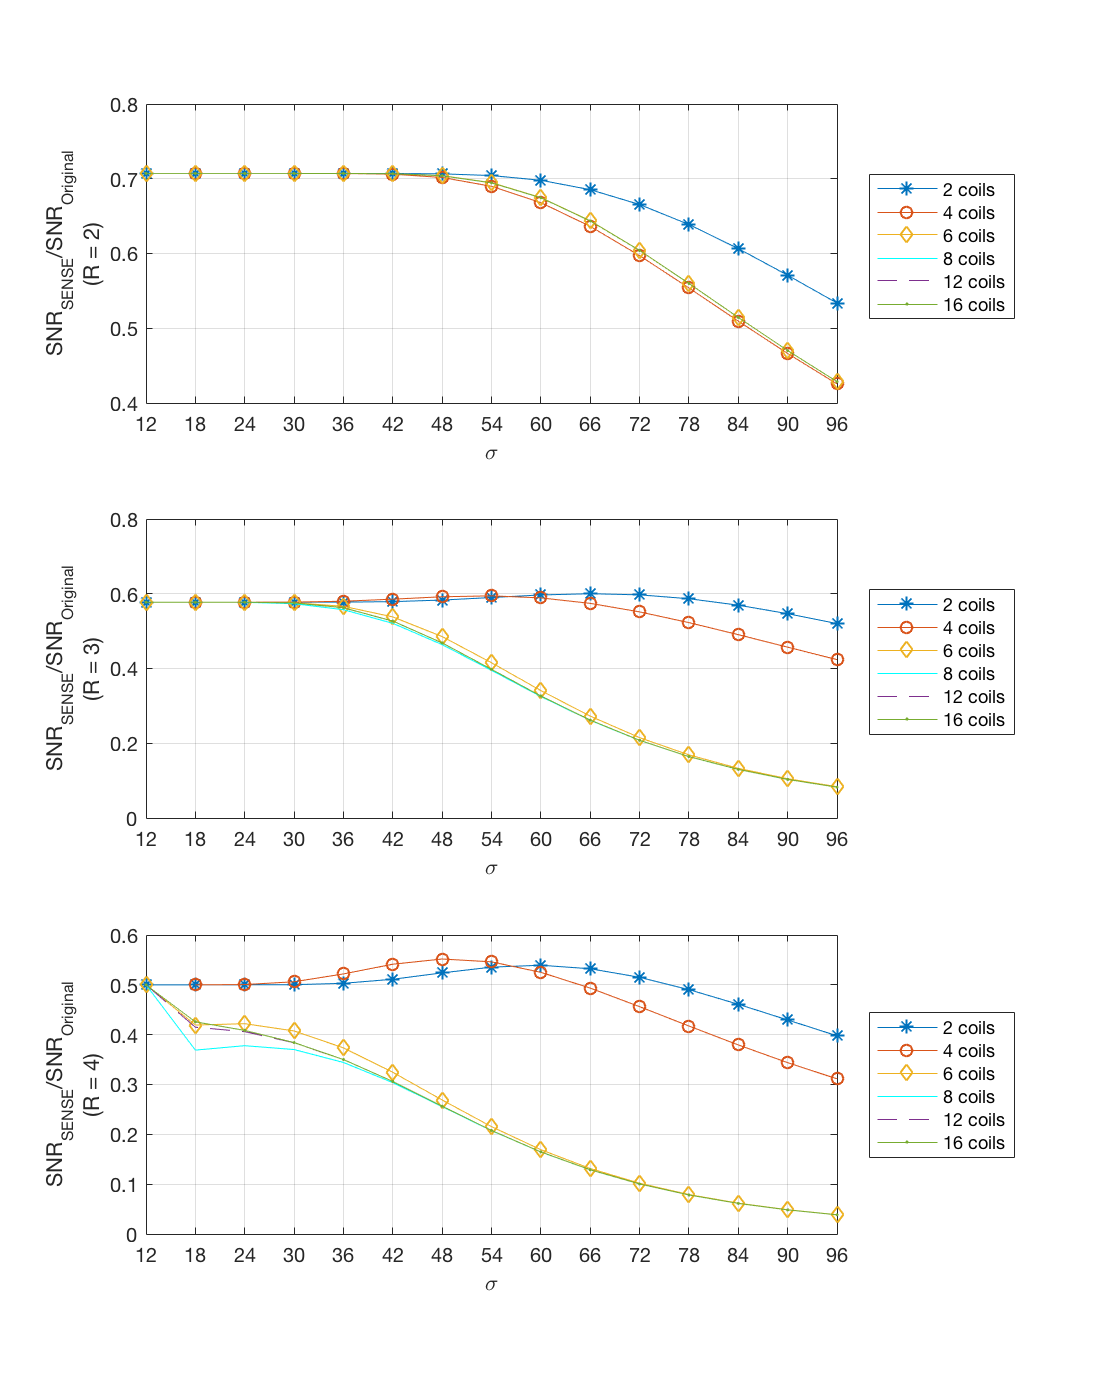
\includegraphics[width=1\textwidth,keepaspectratio]{2SNRsense}
    \caption{The relative decrease in SNR for increasing acceleration factors, coil numbers and standard deviations of the associated sensitivity maps}
    \label{fig:2SNRsense}
\end{figure}


%%%%%%%%%%%%%%%
\section{Influence of noise on SENSE reconstructions}
We have seen so far how SENSE reconstruction is performed with accurate sensitivity maps. However, in a clinical setting, the sensitivity profiles are never perfect and have inherent noise. Moreover, the maps used for reconstruction are acquired during a pre-scan and any patient movement will lead to inaccurate sensitivity profiles and low quality reconstructions. 

Therefore, this section is concerned with reconstructions performed with different levels of noise added to the coil sensitivity maps. The aim of this experiment is to investigate how the quality of reconstruction under these circumstances is affected. One of the major drawbacks of SENSE is not having accurate sensitivity profiles for reconstruction. Errors in these maps will translate into poor reconstructions or even residual aliasing \cite{Deshmane2012}. 

\subsection{Design}
As before, in this experiment we will consider four acceleration factors, different numbers of coils in the array and increasing standard deviations of their associated sensitivity maps. POSSUM simulations were performed with noise-free sensitivity profiles, leaving the white noise addition to the reconstruction step.

The noise was generated from a zero-centered normal distribution $\mathcal{N}(0, \sigma^2)$. We varied the standard deviation of the noise to test the robustness of the reconstruction algorithm and performed simulations for increasing acceleration factors and different numbers of coils. The results can be seen in the following subsection.

\subsection{Results}
As stated before, this experiment is focused on the quality of reconstruction for different levels of noise added to the sensitivity maps. The standard deviation of the normal distribution used to model the noise was ranged from 0 to 2, where for $\sigma = 0$ means no amount of noise is added. More specifically, the values used are: $\sigma_n = \{ 0, 0.001, 0.005, 0.01, 0.05, 0.1, 0.5, 1, 1.5, 2\}$.

The simulations were run for all combinations of coils and for all acceleration factors. The standard deviation of the coil sensitivity profile was set to $\sigma = 48$. The reason behind this decision is that, as can be seen in Figure~\ref{fig:2SSD}, it is one of the points of minimum SSD between accelerated reconstructions and the original image. From this point upward the quality of reconstruction decreases, so it was considered to be a good trade off between all the varying parameters.

The results for SENSE reconstructions are presented in Figures \ref{fig:R1recsnoisej}, \ref{fig:R2recsnoisej}, \ref{fig:R3recsnoisej} and \ref{fig:R4recsnoisej}, whereas the geometry factor maps are presented in Figures \ref{fig:R1gfactnoisej}, \ref{fig:R2gfactnoisej}, \ref{fig:R3gfactnoisej} and \ref{fig:R4gfactnoisej}. Moreover, a sum-of-squared differences was performed between every reconstruction and the original, non-aliased, image. The results are presented in Figure~\ref{fig:ssdnoise}, where every plot shows a different acceleration factor.

\subsection{Discussion}
In this experiment we varied the standard deviation of the noise added to the sensitivity maps used for reconstruction. We then performed SENSE reconstructions for all considered acceleration factors and combinations of coil arrays.

Undoubtedly, the results show that an increase in the level of noise will affect the subsequent reconstructions. The main reason behind this phenomenon is that SENSE-type algorithms rely on accurate sensitivity maps to recover the underlying signal. This is because the first assumption that is made in image based parallel imaging techniques is that every folded spatial location within the aliased images is a juxtaposition of the individual coil sensitivity weighted signal values. Therefore, when the coil maps are changed, the underlying signal can no longer be accurately recovered. This is, of course, directly related to the amount of change brought to these maps, meaning that when the standard deviation of the noise is small, the sensitivity profiles are not changed significantly and relatively accurate reconstructions can still occur. This is also visible in Figures \ref{fig:R1recsnoisej}, \ref{fig:R2recsnoisej}, \ref{fig:R3recsnoisej} and \ref{fig:R4recsnoisej}, where SENSE reconstructions are shown for $\sigma_n$ values between $0$ and $2$.

In fact, as it is presented in Figure~\ref{fig:ssdnoise}, all parameters which were varied in this experiment contribute to a certain extent to the final reconstructions. First, keeping the acceleration factor and the number of coils fixed, it is visible that an increase in noise will directly affect the reconstruction. Clearly, when the acceleration factor is bigger than the number of coils in the array, reconstructions are no longer reliable. That is because in order to unfold aliased locations, one needs at least as many coils as the folded pixels to contribute with the missing information from skipped phase-encoding lines. Second, when the number of receiver channels is increased, the SSD between reconstructions and the original image decreases. This means that when multiple channels are used, reconstructions are more robust to noise. Finally, increasing the acceleration factor leads to worse reconstructions for lower standard deviations of the noise. 
%Actually, this is one of the biggest drawbacks of SENSE-type reconstructions: the need for correct sensitivity profiles of the coils in order to perform as expected and to accurately unfold the aliased images. 

Admittedly, this experiment only shows how different levels of noise added to the sensitivity maps used for SENSE reconstructions affect the quality of the final images. However, two other cases can be identified. First, MRI images are known to be affected by noise. A different experiment would therefore be constructed around accurate sensitivity maps and noisy MRI data, with different levels of noise considered and reconstructions performed for each. Second, as in reality, every piece of electronic equipment has inherent noise, both sensitivity maps and aliased images would have noise added to them. These two scenarios are left for future work.

%% R1
\begin{figure}[H]
    \centering
    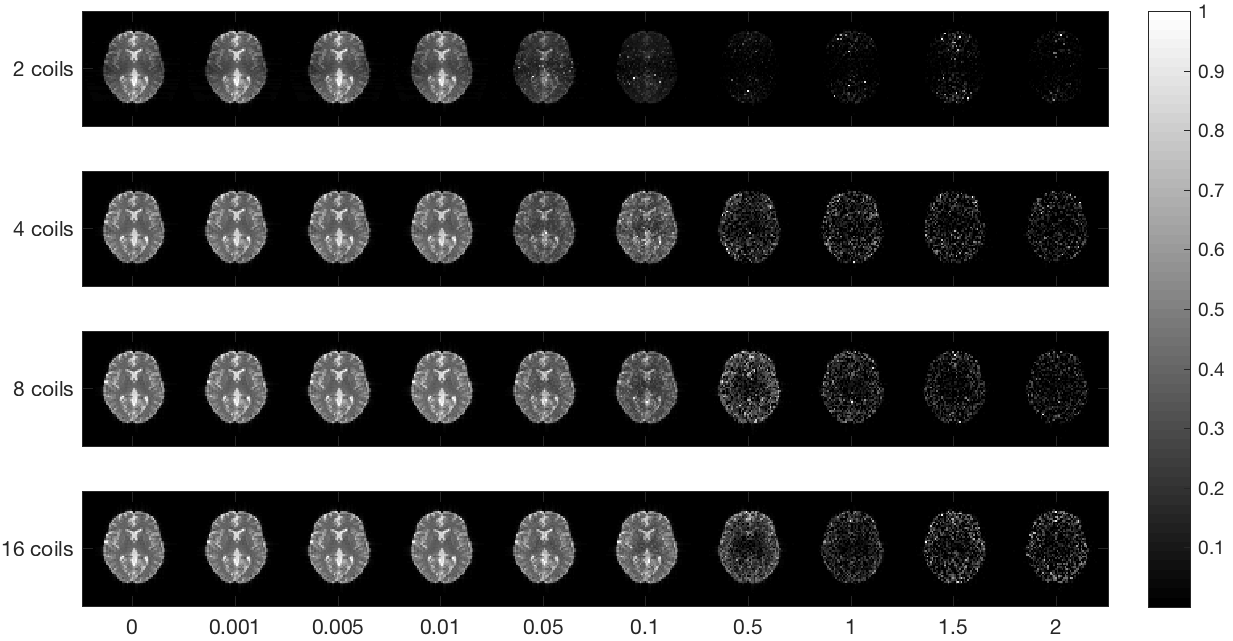
\includegraphics[width=1\textwidth,keepaspectratio]{R1recnoiseb}
    \caption{SENSE reconstructions for acceleration factor $R = 1$, for increasing numbers of coils and for different standard deviations of the noise}
    \label{fig:R1recsnoisej}
\end{figure}

\begin{figure}[H]
    \centering
    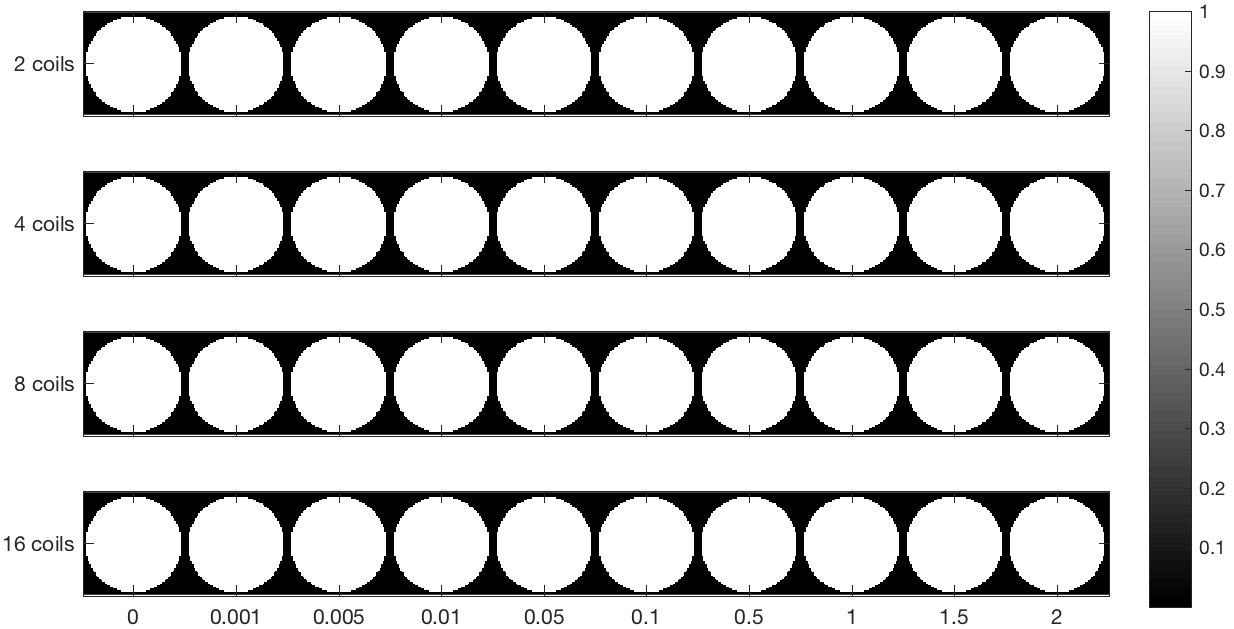
\includegraphics[width=1\textwidth,keepaspectratio]{R1gfactnoiseb}
    \caption{g-factor maps for acceleration factor $R = 1$, for increasing numbers of coils and for different standard deviations of the noise}
    \label{fig:R1gfactnoisej}
\end{figure}

%% R2
\begin{figure}[H]
    \centering
    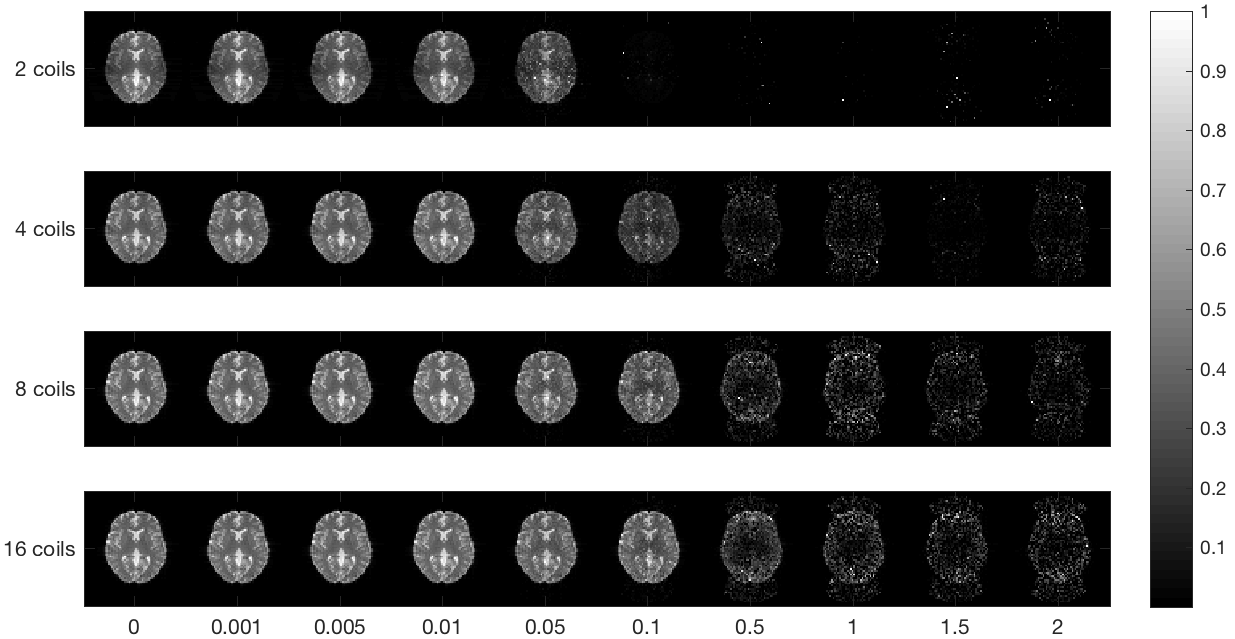
\includegraphics[width=1\textwidth,keepaspectratio]{R2recnoiseb}
    \caption{SENSE reconstructions for acceleration factor $R = 2$, for increasing numbers of coils and for different standard deviations of the noise}
    \label{fig:R2recsnoisej}
\end{figure}

\begin{figure}[H]
    \centering
    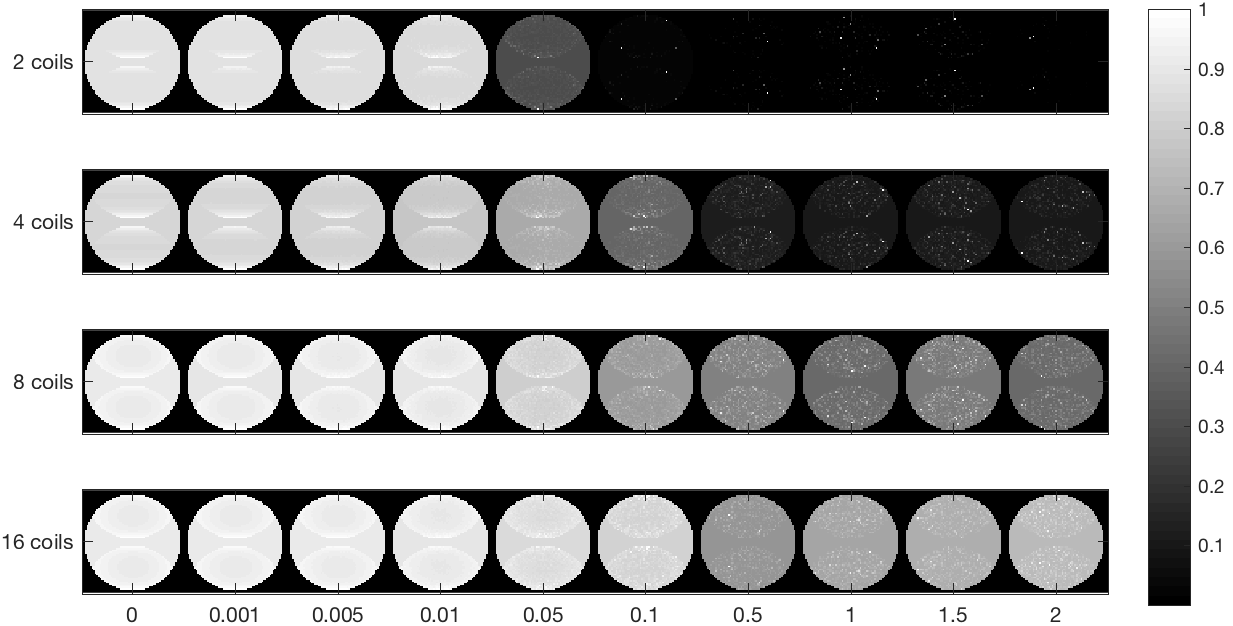
\includegraphics[width=1\textwidth,keepaspectratio]{R2gfactnoiseb}
    \caption{g-factor maps for acceleration factor $R = 2$, for increasing numbers of coils and for different standard deviations of the noise}
    \label{fig:R2gfactnoisej}
\end{figure}

%% R3
\begin{figure}[H]
    \centering
    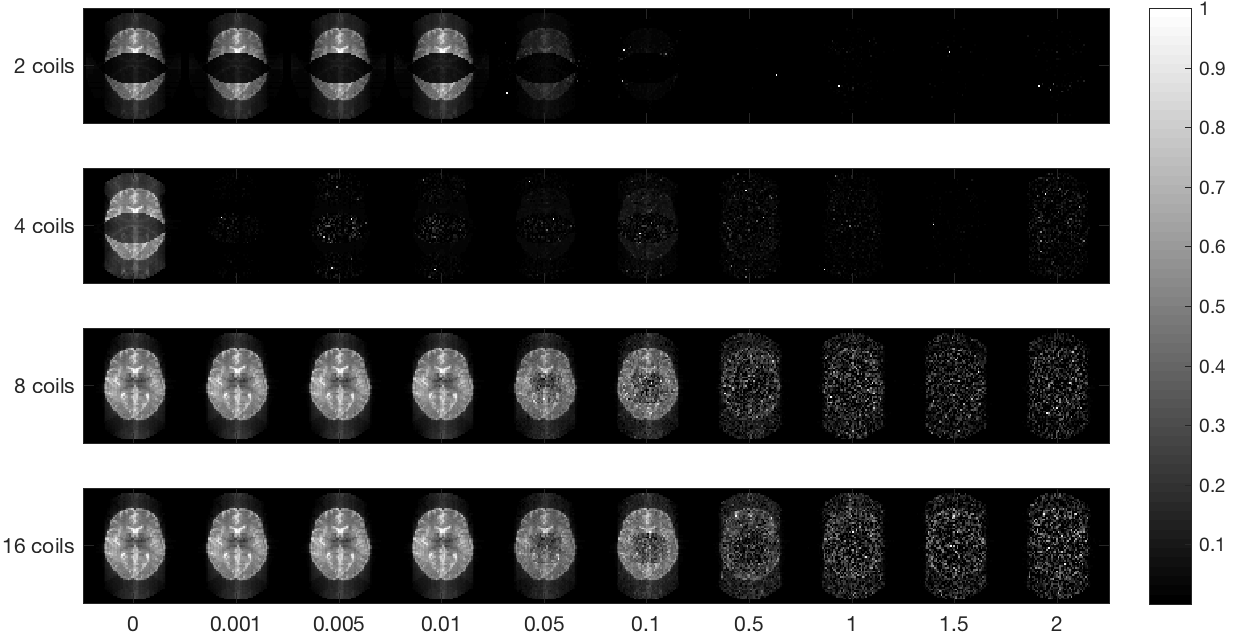
\includegraphics[width=1\textwidth,keepaspectratio]{R3recnoiseb}
    \caption{SENSE reconstructions for acceleration factor $R = 3$, for increasing numbers of coils and for different standard deviations of the noise}
    \label{fig:R3recsnoisej}
\end{figure}

\begin{figure}[H]
    \centering
    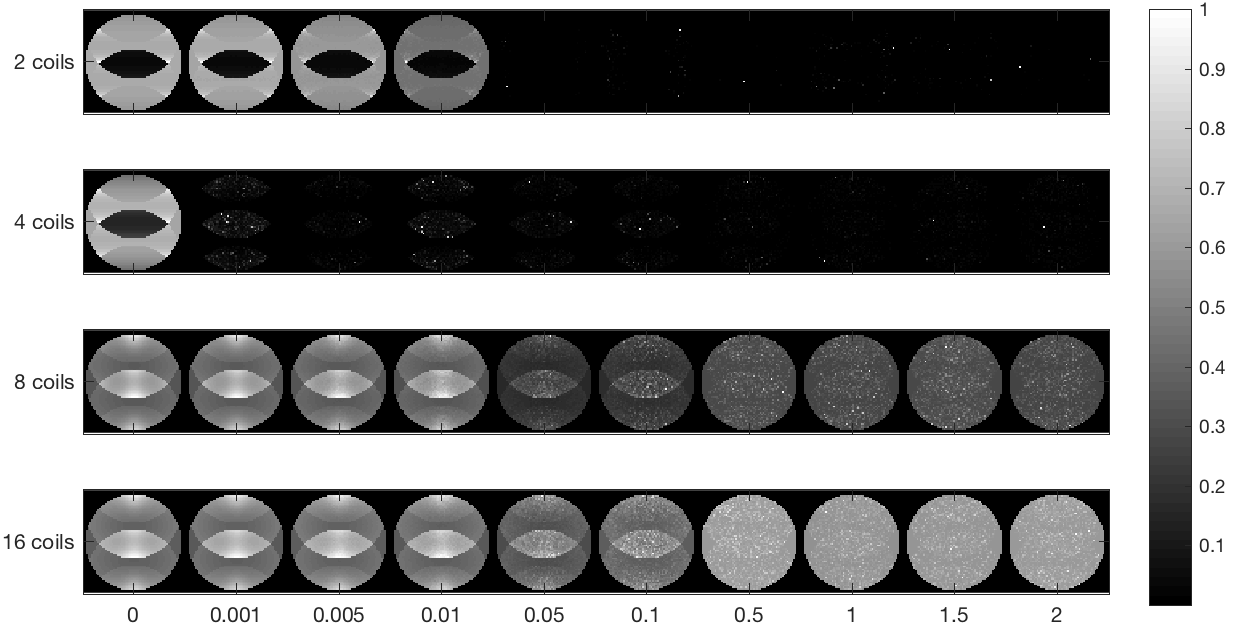
\includegraphics[width=1\textwidth,keepaspectratio]{R3gfactnoiseb}
    \caption{g-factor maps for acceleration factor $R = 3$, for increasing numbers of coils and for different standard deviations of the noise}
    \label{fig:R3gfactnoisej}
\end{figure}

%% R4
\begin{figure}[H]
    \centering
    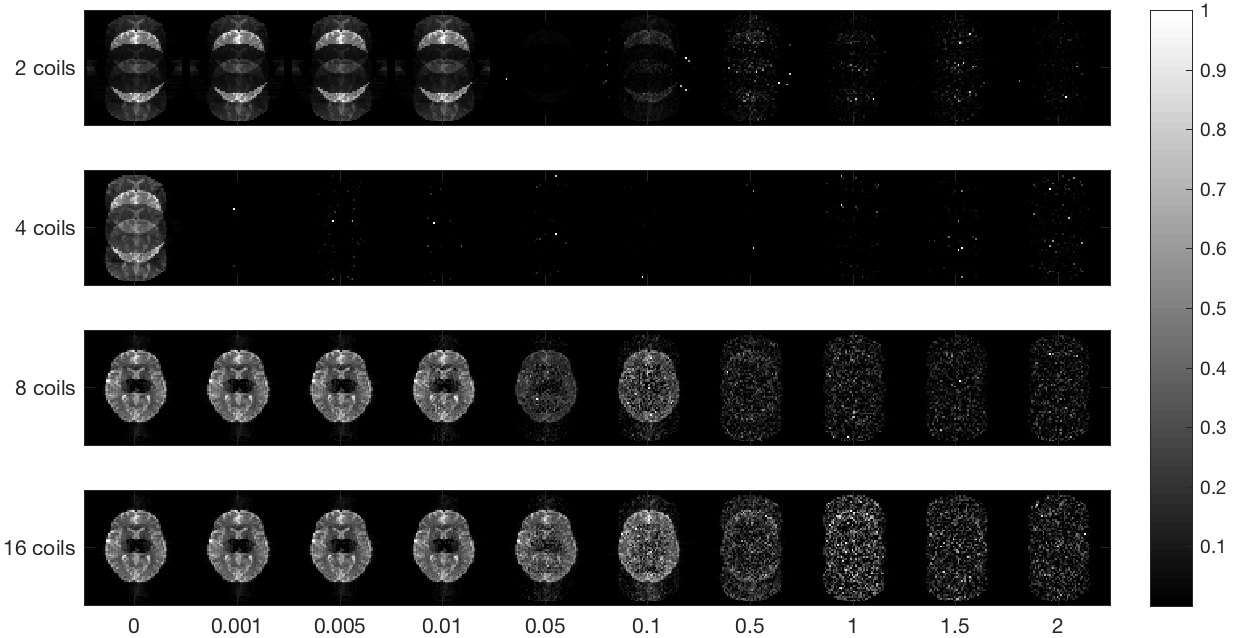
\includegraphics[width=1\textwidth,keepaspectratio]{R4recnoiseb}
    \caption{SENSE reconstructions for acceleration factor $R = 4$, for increasing numbers of coils and for different standard deviations of the noise}
    \label{fig:R4recsnoisej}
\end{figure}

\begin{figure}[H]
    \centering
    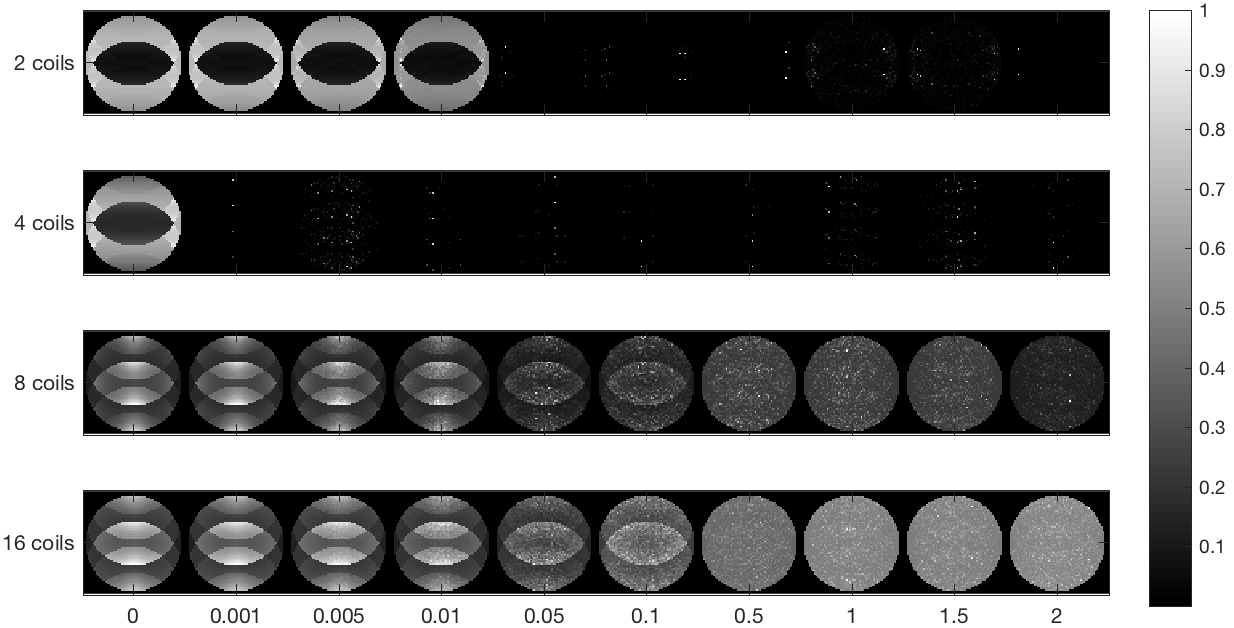
\includegraphics[width=1\textwidth,keepaspectratio]{R4gfactnoiseb}
    \caption{g-factor maps for acceleration factor $R = 4$, for increasing numbers of coils and for different standard deviations of the noise}
    \label{fig:R4gfactnoisej}
\end{figure}

%% SSD
\begin{figure}[H]
    \centering
    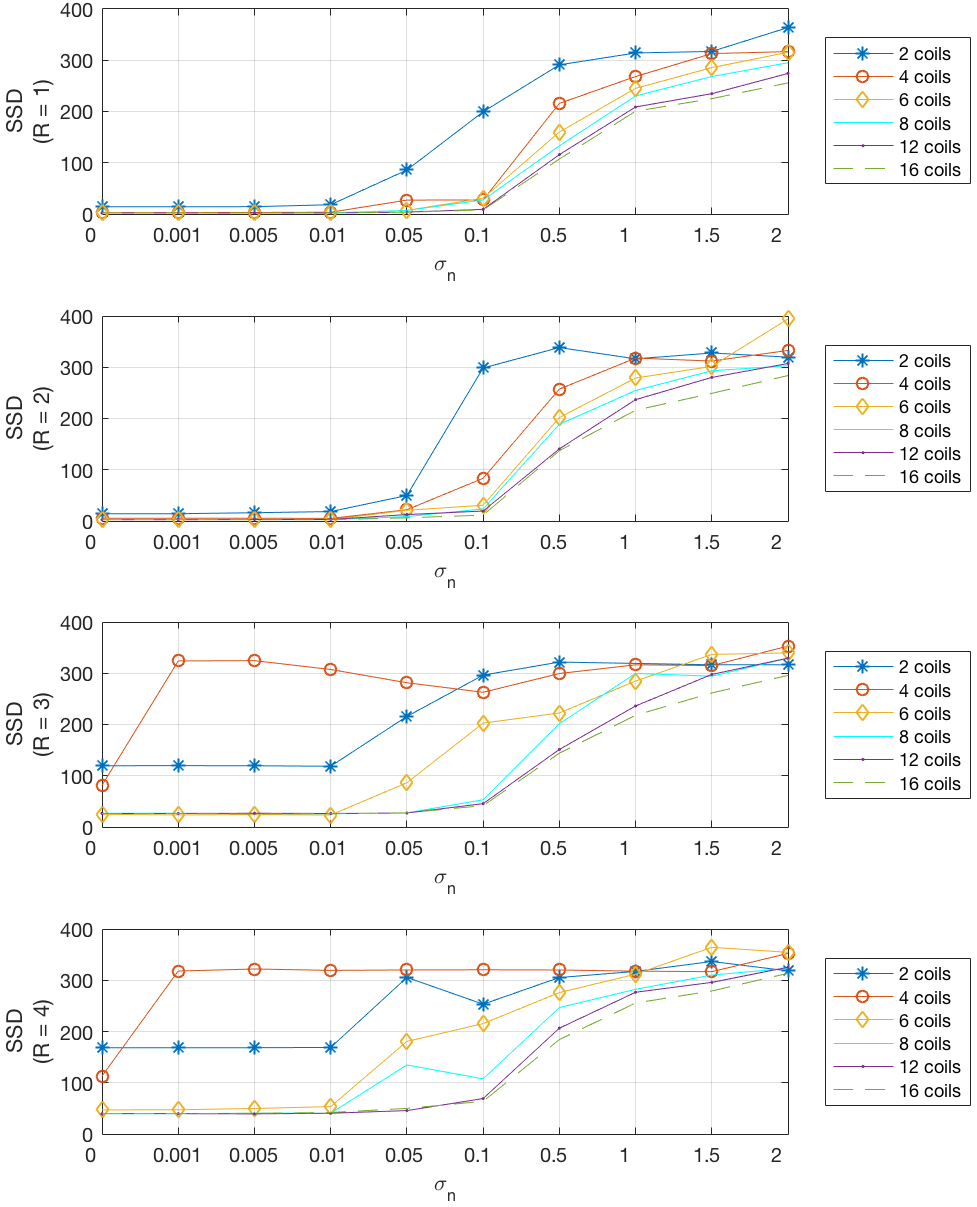
\includegraphics[width=1\textwidth,keepaspectratio]{ssdnoise}
    \caption{SSD between reconstructions and original non-aliased image, for all acceleration factors, for all coil combinations and for all standard deviations of the noise}
    \label{fig:ssdnoise}
\end{figure}

%%%%%%%%%%%%%%%%%%%%%%%%%%%%%%%%
% \section{Motion effects on Parallel Imaging reconstructions}
% Parallel imaging techniques are widely used clinically as they reduce scan time without losing spatial resolution of the final images. This improves patient comfort, is more cost effective and can also reduce motion artifacts. As most MR acquisitions are prone to motion-related artifacts, this section is concerned with investigating the effects of motion when parallel imaging is performed.

% For this, SENSE reconstructions will be performed for different acceleration factors $R = \{1, 2, 3, 4\}$, for all presented channel array combinations (see Figure~\ref{fig:brainsAndCoilsDistrib}) and for all 16 coverage ranges (see Figure~\ref{fig:1coildifsigmas}). Reconstructions will be compared with the original, non-aliased image.

% \subsection{Design}
% In order to simulate motion, POSSUM requires as input a motion sequence file. This file must contain the following parameters, in the specified order: time (in seconds), $T_x$, $T_y$, $T_z$ (translations along all 3 axis, in meters) and $R_x$, $R_y$, $R_z$ (rotations about the specified axis, in radians). For this experiment, a motion file was designed such that the object rotates about the z-axis (yaw) starting from a certain time point. This design choice was made in order to see that parallel imaging techniques, as they require less time to acquire the data, will no longer be affected by the object's movements. The motion file is plotted in Figure~\ref{fig:motioniri}.

% \begin{figure}[H]
%     \centering
%     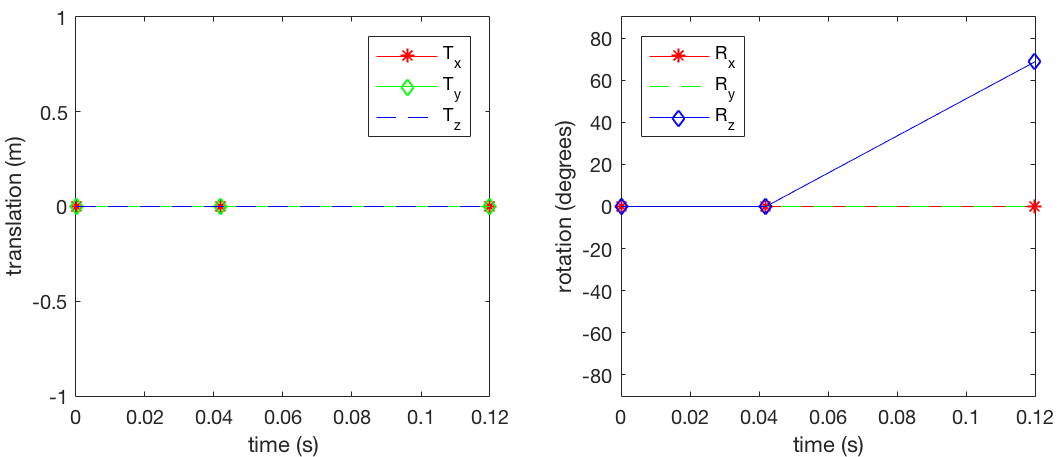
\includegraphics[width=1\textwidth,keepaspectratio]{motioniri}
%     \caption{Motion sequence file}
%     \label{fig:motioniri}
% \end{figure}

% When simulations are performed with acceleration factor $R = 1$, the 64 phase-encoding lines of k-space are acquired in 50ms, while the middle k-space is being acquired after the first 30ms ($TE_{eff} = 0.03s$). However, increasing acceleration factors will shorten the echo train making it less likely for the acquisition to be affected by motion. In this experiment we investigate whether this scenario holds true.

% As can be seen in Figure~\ref{fig:motioniri}, the motion sequence was designed to start after $TE_{eff}$, but before the end of the $R = 1$ slice acquisition. As the object (the brain, in our case) will rotate only during the latter part of the acquisition, blurring will be seen in the final image. As more than half of k-space lines were acquired when no motion was involved, the reason behind the blurring comes from the faulty lines acquired during motion. Figure~\ref{fig:motionvsnomotion} shows the motion corrupted image, as well as the no motion case and the absolute difference between the two.

% \begin{figure}[H]
%     \centering
%     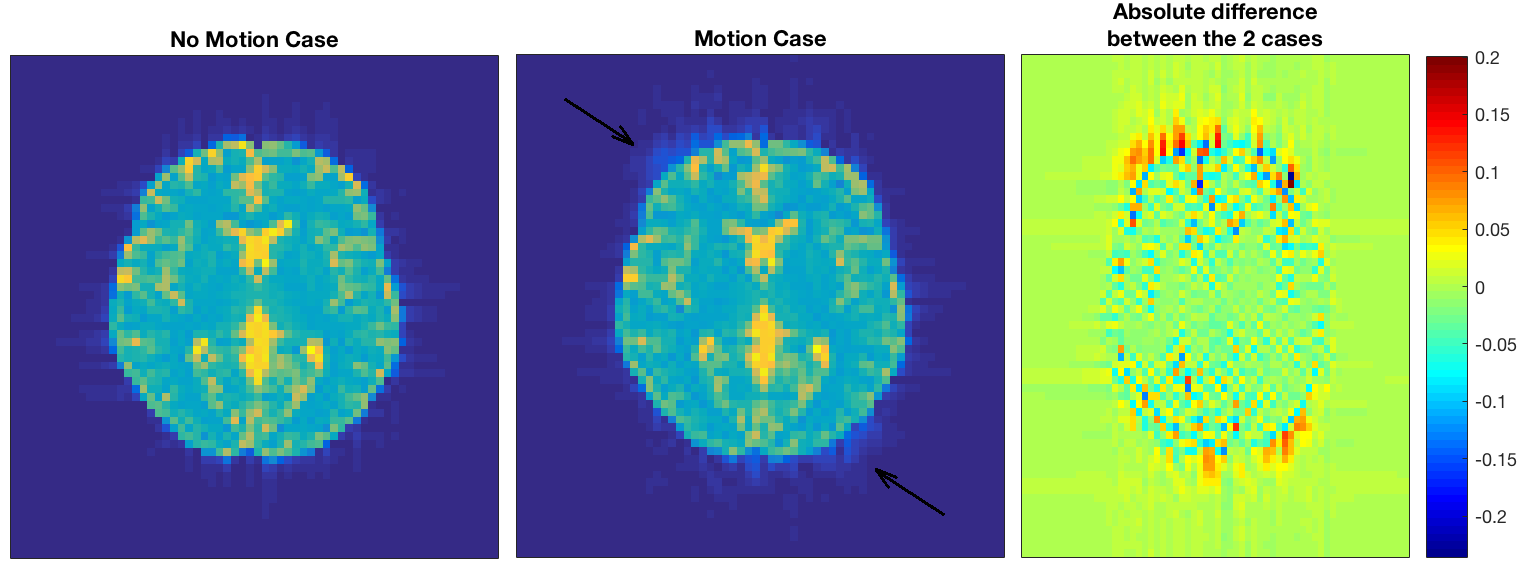
\includegraphics[width=1\textwidth,keepaspectratio]{motionvsnomotion}
%     \caption{The two cases are presented: the no motion case can be seen in the left hand side of the figure, the motion corrupted case is found in the middle image, and the absolute difference between the two is presented in the right hand side of the figure. The blurring artifact is visible in the middle image.}
%     \label{fig:motionvsnomotion}
% \end{figure}

% For this experiment, simulations were run for all 4 acceleration factors, all 6 coil combinations and all 16 sensitivity maps. A region of interest was chosen on the final images and a sum-of-squared differences was performed between all reconstructions and the no motion case. These results were compared with the SSD between the motion case and no motion when parallel imaging was not used. The reason for this was to see that with higher acceleration factors, the reconstructions will be less prone to motion and therefore more close to the no motion case.

% \subsection{Results}
% Motion during MRI scans causes the excited spins to change position between phase-encoding gradients and signal reading. As a result, motion artifacts appear in the final images mainly in the phase-encoding direction. For this reason, the region of interest chosen in this experiment spans across the y-direction more so than across the x-direction. Figure \ref{fig:brainroi} shows the ROI in both the motion and no motion cases.

% \begin{figure}[H]
%     \centering
%     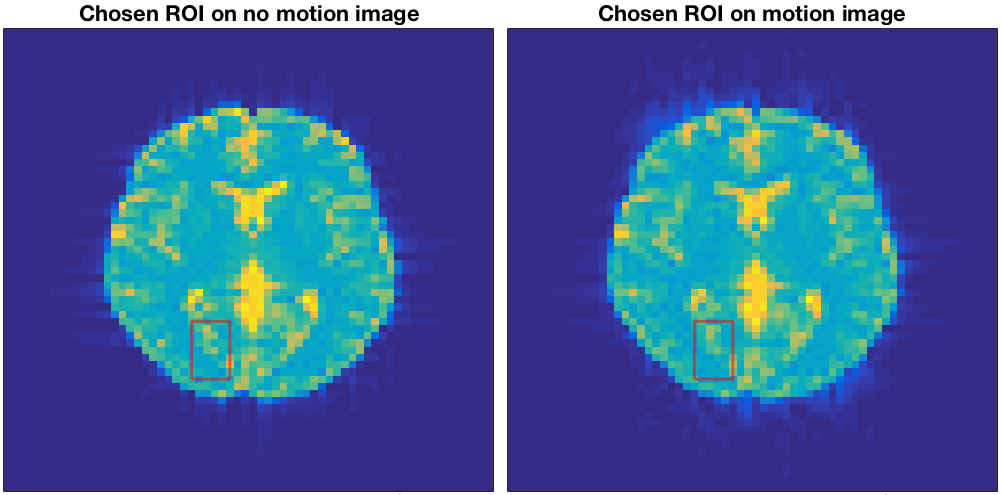
\includegraphics[width=1\textwidth,keepaspectratio]{brainroi}
%     \caption{The chosen ROI shown for both motion and no motion cases}
%     \label{fig:brainroi}
% \end{figure}

% As stated before, simulations were run for the motion case for all acceleration factors, all coil combinations and all sensitivity maps. Figure \ref{fig:resultsexp4} shows the results of this experiment. Each plot represents a different acceleration factor $R$, while the x-axis of these plots represents the standard deviations of the sensitivity profiles, in increasing order. The y-axis is in logarithmic scale and represents the sum-of-squared differences between the reconstructions and the no motion original image. Moreover, the green line shown in each plot represents the SSD between the motion and no motion cases presented in Figure~\ref{fig:motionvsnomotion}.

% The best results can be seen in the second plot, where acceleration factor $R = 2$. The SENSE reconstruction for the 2-coil array, for $\sigma = 72$ is shown in Figure~\ref{fig:bestrec}. The other combinations of parameters show promising results as well, although, when $\sigma < 72$, the reconstructions do not perform well enough. Moreover, the simulations performed with $R > 2$ do not perform as well due to ill-conditioned reconstructions. These drawbacks of the method were presented in Section \ref{exp2}. 

% \begin{figure}[H]
%     \centering
%     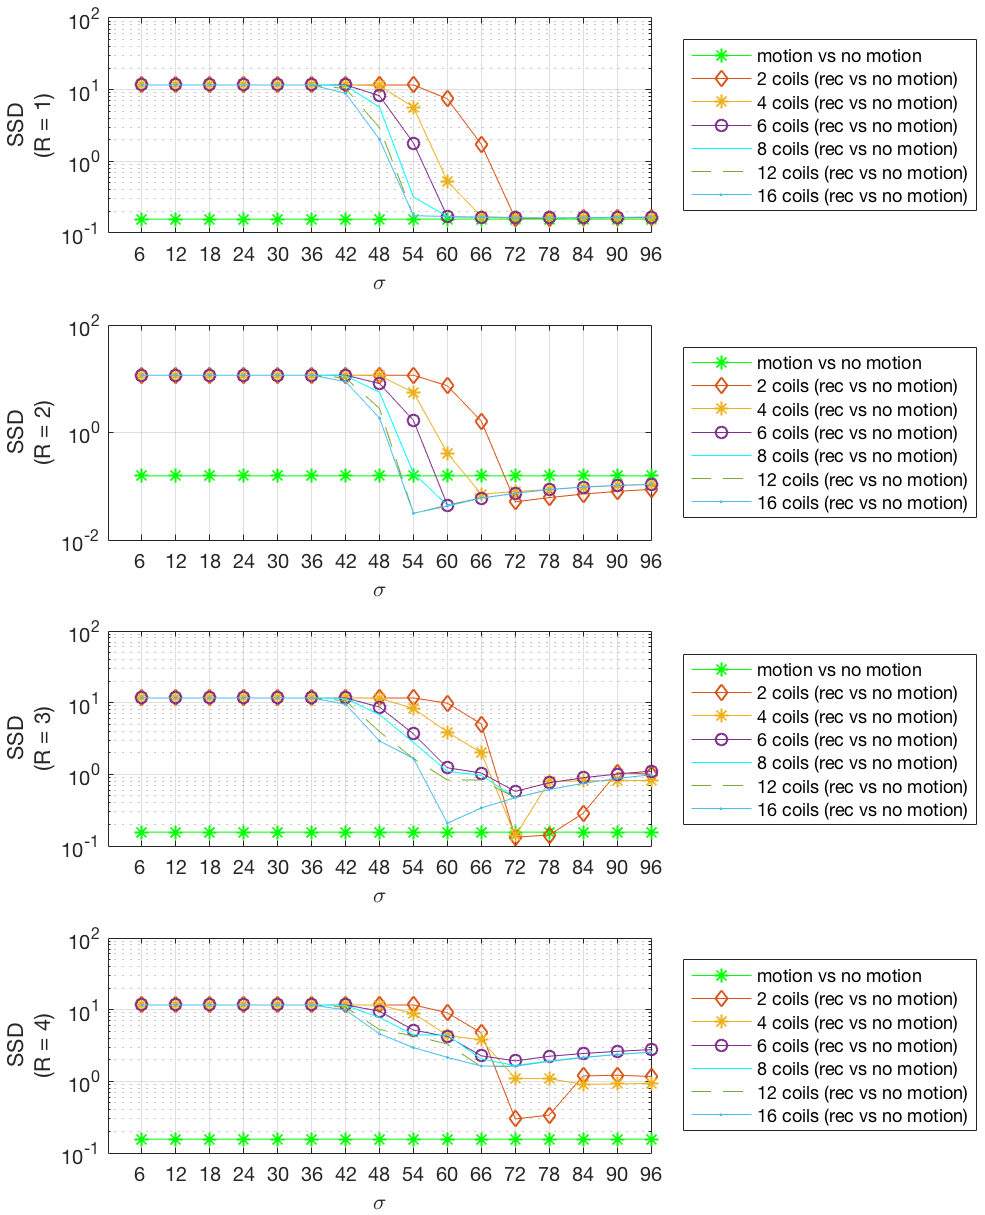
\includegraphics[width=1\textwidth,keepaspectratio]{resultsexp4all}
%     \caption{SSD between reconstructions and original non-aliased image, for all acceleration factors, for all coil combinations and for all standard deviations of the sensitivity profiles. In green, the SSD between the original non-aliased image and the original motion simulated image is shown. All values shown are for a chosen ROI as presented in Figure \ref{fig:brainroi}}
%     \label{fig:resultsexp4}
% \end{figure}

% \begin{figure}[H]
%     \centering
%     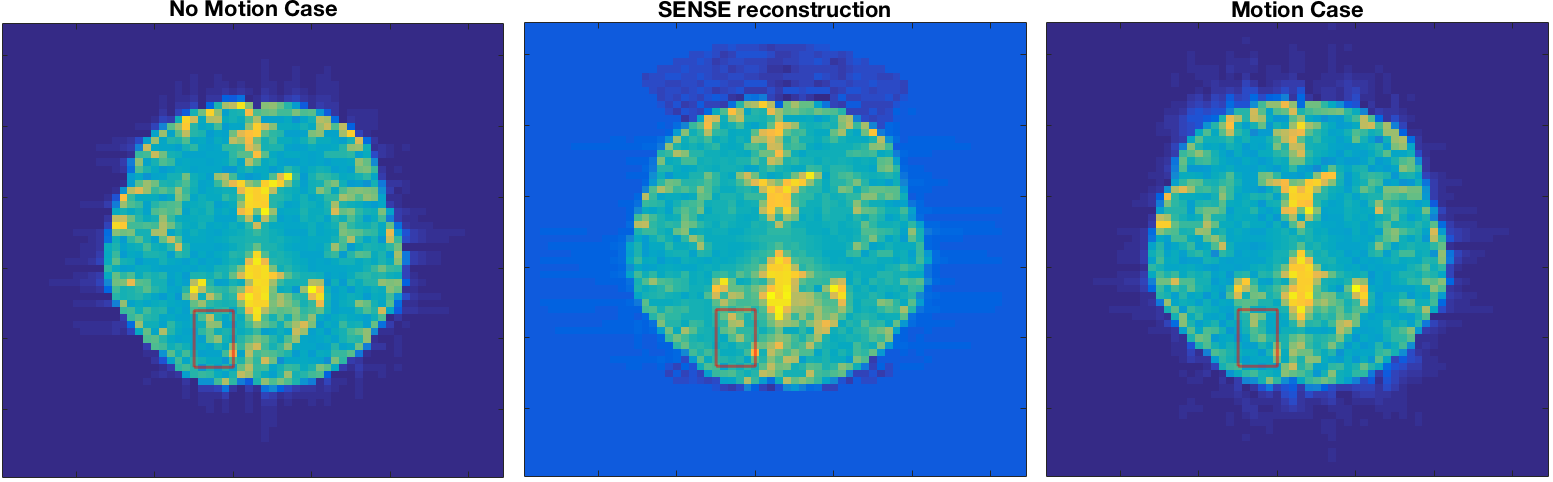
\includegraphics[width=1\textwidth,keepaspectratio]{bestrec}
%     \caption{The no motion and motion cases are shown in the left hand side and the right hand side of the image, while SENSE reconstruction for $R = 2$, $\sigma = 72$ and a 2 coil channel array is shown in the middle}
%     \label{fig:bestrec}
% \end{figure}

% \subsection{Discussion}
% In this experiment, a motion sequence was defined and used as input to our simulations in order to investigate the effect of object movement when parallel imaging is performed for various acceleration factors. Figure~\ref{fig:motionvsnomotion} shows the SSD between all SENSE reconstructions and the original non-aliased image. 

% First, it is visible from the plot that when no acceleration is in place, meaning $R = 1$, the reconstruction resembles the motion case as presented in Figure~\ref{fig:motionvsnomotion}. For the first 9 standard deviations of the sensitivity maps, the reconstruction is poor as the coil profile's coverage is not large enough to encompass the necessary field-of-view. For the last 7 sensitivity profiles, reconstruction can be performed. As all SENSE reconstructions are basically the original, motion simulated image, the SSD between the chose ROIs will be the same as the SSD between the two original cases, when parallel imaging is not involved.

% Second, when acceleration factor 2 is used, the echo train becomes small enough that it does not encompass the motion anymore. That is clearly visible from the second plot where all reconstructions, for the sensitive enough coil profiles, perform better in terms of SSD than the original motion simulated image. 

% Finally, when higher acceleration factors are used, as was presented in Section \ref{exp2}, the quality of reconstruction drops significantly. Moreover, when $R > 2$ and an array with 2 channels is used, reconstructions cannot be performed as the number of juxtaposed signals in the aliased images is greater than the available coil information. Thus, the results show an outlier which just happened to be closer to the original non-aliased image, making the SSD drop significantly.

% All in all, this has been a proof of concept experiment. It is evident from the results shown that motion is a highly complicated aspect of MRI simulation that requires more cases than the one presented. First of all, motion was present for less than half of the k-space acquisition time. As movement can happen throughout the read-out period, an experiment involving motion throughout the whole signal acquisition should be considered. Second, reconstructions for $R > 2$ did not perform well to begin with, making this experiment less likely to show major improvements for such cases. Next, the conclusions and future work will be presented.

















